\documentclass[hyperpdf,bindnopdf,11pt]{hepthesis}

\usepackage{xspace}
\usepackage{hepnames}
\usepackage{hepunits}

% Acronyms
\newcommand{\CMS}{CMS\xspace}
\newcommand{\ATLAS}{ATLAS\xspace}
\newcommand{\LHC}{LHC\xspace}
\newcommand{\CERN}{CERN\xspace}
\newcommand{\WLCG}{WLCG\xspace}
\newcommand{\ECAL}{ECAL\xspace}
\newcommand{\HCAL}{HCAL\xspace}
\newcommand{\LINACTWO}{LINAC2\xspace}
\newcommand{\PSBooster}{PS Booster\xspace}
\newcommand{\PS}{PS\xspace}
\newcommand{\SPS}{SPS\xspace}
\newcommand{\BSM}{BSM\xspace}

% Physics symbols
\newcommand{\lumi}{\ensuremath{\mathcal{L}}\xspace}
\newcommand{\mom}{\ensuremath{p}\xspace}
\newcommand{\pt}{\ensuremath{\mom_{\text{T}}}\xspace}
\newcommand{\dphi}{\ensuremath{\Delta\phi}\xspace}
\newcommand{\deta}{\ensuremath{\Delta\eta}\xspace}

% Math shorthand
\newcommand{\aeta}{\ensuremath{|\eta|}\xspace}



%% PDF metadata
\makeatletter
\@ifpackageloaded{hyperref}{%
    \hypersetup{%
        hidelinks=true,
        pdftitle = {Precision measurement of the Z invisible width with the CMS experiment}
        pdfsubject = {Shane Breeze's PhD thesis},
        pdfkeywords = {CMS, Electroweak physics, Z boson, Precision measurement, LHC},
        pdfauthor = {\textcopyright\ Shane Breeze},
        linkcolor=black,
        colorlinks=false
    }
}{}
\makeatother

\renewcommand{\listfigurename}{List of figures}
\renewcommand{\listtablename}{List of tables}

\title{Precision measurement of the \PZ invisible width with the \CMS experiment}
\author{Shane Breeze}

%\includeonly{chapters/100_appendices/appendices,chapters/200_biblio/biblio}
\includeonly{chapters/031_reconstruction/reconstruction,chapters/200_biblio/biblio}

\begin{document}

    \begin{frontmatter}
        \titlepage[Imperial College London\\Department of Physics]{
    A dissertation submitted to Imperial College London\\
    for the degree of Doctor of Philosophy
}

        \begin{abstract}
    Abstract
\end{abstract}

        \begin{declaration}
    Declaration
\end{declaration}

        \begin{acknowledgements}
    Cheers Baker.
\end{acknowledgements}

        \begin{preface}
    Preface
\end{preface}

        \tableofcontents
\listoffigures
\listoftables
%\frontquote{}{}

    \end{frontmatter}

    \begin{mainmatter}
        \cleardoublepage
        \pagenumbering{arabic}
        \chapter{Introduction}
\label{chap:introduction}

\pagenumbering{arabic}
%\chapterquote{}{}

The classification and description of fundamental particles and their
interactions by the standard model (SM) of particle physics has been
successfully confirmed by countless experiments. However, it lacks a
candidate for dark matter \cite{Ade:2015xua,Corbelli:1999af}, a neutrino
oscillation mechanism \cite{Fukuda:1998ah,Ahmad:2002jz,Eguchi:2002dm}, or
incorporating the gravitational interaction. At the LHC, the SM gained further
success upon the discovery of the Higgs boson
\cite{Aad:1471031,Chatrchyan:1471016}. Although numerous direct searches for
beyond the SM (BSM) have been performed, no clear signal of BSM physics has
been observed. As these searches continue to probe the extremities of
distributions for BSM physics, an alternative direction proceeds through
precision measurements of the SM, as presented in this thesis.

The SM predicts that about $20\%$ \cite{PhysRevD.98.030001} of the time a \PZ
boson decays into a neutrino-antineutrino pair. This decay constitutes the \PZ
invisible width, a signal not discernible in collider-based experiments.
Instead, it is inferred from the missing momentum associated with the invisible decay of the \PZ as it recoils against a detectable system. A measurement of the \PZ invisible width is a key test of the SM and can be translated into constraints on the number of neutrino species coupling to the \PZ boson. Deviations from the SM expectation may point towards the existence of new particles beyond the SM which contribute to the \PZ invisible width. Therefore, a precise measurement of this quantity could reveal signs of new physics

The experiments at LEP measured the invisible width of the \PZ using two
methods. The direct method measures the rate of an energetic photon recoiling
against an invisible system attributed to the s-channel \PZ production and
subsequent invisible decay with an associated initial state radiated (ISR)
photon: $e^+e^-\ra \gamma Z \ra \gamma\nu\bar{\nu}$. The indirect method
measures the total \PZ width, by studying the lineshape of the \PZ boson from
$e^+e^-$ collisions with a centre of mass energy near the \PZ mass, and
subtracts the partial widths to all visible final state. This method provides
the most precise measurement, with a sensitivity to BSM particles. A summary
of the measurements performed by the LEP experiments L3
\cite{Acciarri:1998vf}, OPAL \cite{Akers:1994vh} and ALEPH
\cite{Buskulic:1993ke} for the direct method, a combination and the indirect
measurement is shown in Tab.~\ref{tab:lep-zinv-width}.

\begin{table}[htb]
    \centering
    \begin{tabular}{cc}
         \hline\hline
         Experiment & $\Gamma_{\mathrm{inv}}$ (MeV) \\
         \hline
         L3 & $498\pm 12\pm 12$ \\
         OPAL & $539\pm 26\pm 17$ \\
         ALEPH & $450\pm 34\pm 34$ \\
         LEP combined & $503\pm 16$ \\
         \hline
         LEP indirect & $499.0\pm 1.5$ \\
         \hline
    \end{tabular}
    \caption{
        Summary of the measurements of the $\Gamma_{\mathrm{inv}}$ from the LEP experiments for the direct measurements (with the statistical and systematic uncertainties), its combination, and the indirect measurement.
    }
    \label{tab:lep-zinv-width}
\end{table}

To date, there is no published measurements of the \PZ invisible width at a
hadron collider. However, a precise measurement at the LHC complements the LEP
measurements through an independent test of the SM at a different energy
scale, exposing contributions to the invisible width to TeV scale
contributions. These additional contributions may come from couplings of the
\PZ with dark matter particles, such as the lightest supersymmetric candidate,
or a mixing between the neutrino and sterile neutrino states
\cite{Carena:2003aj}, to which both the direct and indirect measurements are
sensitive. However, the direct measurement is also sensitive to
contributions to the invisible final state without coupling to the \PZ boson,
such as a heavier mediator coupling to neutrinos or other exotic invisible
particles, or a four fermion interaction vertex \cite{Carena:2003aj}.
Therefore, both measurements are valuable tests of the SM with the direct
measurement a candidate for the LHC to provide a complementary measurement.

The experiment and analysis presented by the author is a direct measurement of
the invisible width of the \PZ boson with the CMS detector using data from
proton-proton collisions at ${\sqrt{s}=\SI{13}{TeV}}$ in 2016, corresponding
to an integrated luminosity of $\SI{35.9}{fb^{-1}}$. The measurement targets
the invisible decay of the \PZ bosons recoiling against a hadronic system. The
rate of the invisible final state is compared to the reference signal of the
partial widths to leptons (both electrons and muons) $\Gamma(\PZ\ra\ell\ell)$, since these decays are
kinematically similar. The invisible width is then given by
%
\begin{equation}\label{eq:zinv}
    \Gamma(\IZinv) = \frac{\sigma(\IZj)\mathcal{B}(\IZinv)}{\sigma(\IZj)\mathcal{B}(\IZll)}\Gamma(\IZll)\ ,
\end{equation}
%
where $\sigma(\IZj)$ is the cross section for the \IZj process, modified by
either the invisible branching fraction $\mathcal{B}(\PZ\ra\mathrm{inv.})$ or
dilepton branching fraction $\mathcal{B}(\IZll)$.
        \chapter{The Standard Model of Particle Physics}
\label{chap:theory}

%\chapterquote{}{}

\section{Introduction}

The standard model (SM) of particle physics is a quantum field theory description of the fundamental particles of matter and their interactions. The SM has been widely successful in its predictions, falling short in providing a dark matter candidate, including the existence of neutrino oscillations and incorporating gravitational interactions, among other possible discrepancies.  Nevertheless, it is the current best minimal description unifying the electromagnetic, weak and strong forces. In the quantum field theory, the equations of motion are determined from the Lagrangian through the principle of least action. Gauge theories provided the mathematical basis to embed physical symmetries within the model.

The SM has had many distinguishing successes since its conception. One of the most notable is the prediction of the Higgs boson \cite{PhysRevLett.13.321,PhysRevLett.13.508,PhysRevLett.13.585} and its subsequent discovery by the ATLAS \cite{Aad:2012tfa} and CMS \cite{Chatrchyan:2012xdj} experiments. The Higgs field is crucial in providing a mechanism for the apparent masses of the weak bosons, quarks and charged leptons whilst maintaining a gauge invariant theory.

This chapter will include an overview of the properties of the SM with particular detail on the quantum electrodynamic, quantum chromodynamic and electroweak sectors, leading to a discussion of the spontaneous symmetry breaking in the SM, known as the Higgs mechanism. This is followed by a discussion of the Monte Carlo techniques used to simulate the SM.


\section{Elementary particles}

The set of fundamental particles and interaction mediators within the SM is shown in Fig.~\ref{fig:particle}. This includes the quarks --- fermion constituents of protons and neutrons --- with three generations of up and down-type quarks with a charge of $+2/3$ and $-1/3$ (in units of the elementary charge). A quark also takes one of three colour states, the strong force equivalent of the electric charge. Through these colour states the quarks interact with the gluon colour octet via the strong interaction. In addition, the lepton sector consists of charged fermions which, in addition to the quarks, interact through the photon field leading to the electromagnetic interaction. Furthermore, all fermions --- quarks, charged leptons and neutral leptons (neutrinos) --- interact via the weak force, mediated by the \PW and \PZ bosons. A set of antiparticles mirror all the fermions leading to 12 fermion fields and an equal number of anti-fermion fields, split into 6 quarks and 6 leptons.

\begin{figure}[htb]
    \centering
    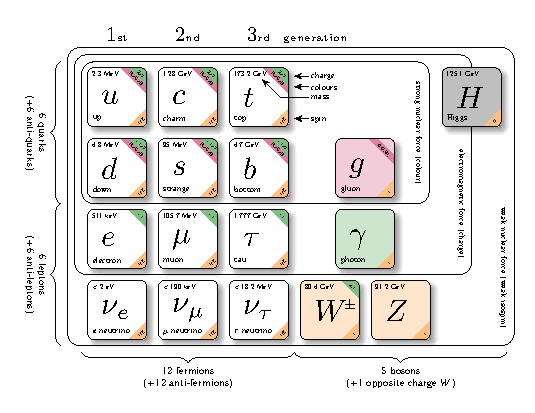
\includegraphics[width=0.8\textwidth]{diagrams/tikz/standard_model/standard_model.pdf}
    \caption[Summary of the standard model particles.]{
        Diagram of the particles within the SM including their quantum numbers such as charge, colour and spin, along with their measured masses. The left and right-handed chiral states are omitted and left for discussion in the main text.
    }
    \label{fig:particle}
\end{figure}


\section{Gauge theories}

In quantum field theory, the fundamental fields are unobservable. Instead, properties deriving from these fields, such as the cross section or rate of an interaction or decay, are measured. Many configurations of the underlying fields can give identical observable quantities. The transformation between these configurations is known as a gauge transformation and leaves the physical observables unchanged, hence these transformations are known as gauge invariant. Under Noether's theorem, a change in the field configuration which leaves the action, and hence the Lagrangian density, invariant is associated with conserved currents \cite{doi:10.1080/00411457108231446}.

\subsection{Quantum Electrodynamics}

Quantum electrondynamics (QED) is a gauge theory that sets out to describe the electron and the photon along with their interactions. The QED Lagrangian density consists of a Dirac field, the electron; a vector field, the photon, derived from Maxwell's equations; and an interaction term between the electron and photon fields:
%
\begin{equation}
    \mathcal{L}_{\mathrm{QED}} = \mathcal{L}_{\mathrm{Dirac}} + \mathcal{L}_{\mathrm{Maxwell}}\ + \mathcal{L}_{\mathrm{int}}\ .
\end{equation}

Maxwell's equations of electromagnetism are obtained from the Euler-Lagrange equations applied to the Lagrangian
%
\begin{equation}
    \mathcal{L}_{\mathrm{Maxwell}} = -\frac{1}{4}F^{\mu\nu}F_{\mu\nu}\ ,
\end{equation}
%
where $F^{\mu\nu}=\partial^{\mu}A^{\nu}-\partial^{\nu}A^{\mu}$ \cite{Peskin:1995ev} for the 4-potential $A^{\mu}$ with an electric scalar potential time-like and magnetic vector potential space-like components.

The Dirac Lagrangian describes the equations of motion, through application of the Euler-Lagrange equations \cite{Troutman1983}, of a spin-half fermion field $\psi$. This field is represented as a four-component spinor which may be interpreted as the spin-up and down of the left and right-handed helicity states \cite{Peskin:1995ev}. To form Lorentz invariant quantities, required in the Lagrangian, the adjoint field is defined as $\bar{\psi}=\psi^{\dagger}\gamma^0$ where $\psi^{\dagger}$ is the Hermitian conjugate of $\psi$ and $\gamma^0$ is the time-like component of the Dirac gamma matrices. These matrices obey the anticommutation relation $\{\gamma^{\mu},\gamma^{\nu}\} = 2g^{\mu\nu}$, where $g^{\mu\nu}$ is the Minkowski space metric, leading to the Lorentz invariant quantities such as $\bar{\psi}\psi$ and $\bar{\psi}\gamma^{\mu}\psi$ \cite{Peskin:1995ev}. These quantities form the basis of the Dirac Lagrangian of a free spin-half fermion:
%
\begin{equation}
    \mathcal{L}_{\mathrm{Dirac}} = i\bar{\psi}\gamma^{\mu}\partial_{\mu}\psi - m\bar{\psi}\psi\ ,
\end{equation}
%
where $i\partial_{\mu}$ is the position-space representation of the 4-momentum $p_\mu$, and $m$ is the mass of the particle \cite{1928RSPSA.117..610D}.  $U(1)$ group transformations of the field
%
\begin{equation}
    \psi \mapsto e^{i\alpha}\psi
\end{equation}
%
are not physical observables since they cancel in the magnitude of the matrix element used to determine the rate or cross section of a process. The Lagrangian is already invariant to such global transformations. However, local transformations where $\alpha\mapsto\alpha(x)$ introduces a term to the Dirac Lagrangian given by
%
\begin{equation}
    \mathcal{L}_{\mathrm{Dirac}} \mapsto \mathcal{L}_{\mathrm{Dirac}}  - \bar{\psi}\gamma^{\mu}(\partial_\mu\alpha(x))\psi\ ,
\end{equation}
%
To enforce gauge invariance, this additional term must be removed by introducing an additional field to the Dirac Lagrangian with a $U(1)$ transformation which opposes the additional term. Therefore, a $U(1)$ gauge invariant electron field must include an interaction with this new field, which is the photon field. This interaction term is realised through gauge invariance as
%
\begin{equation}
    \mathcal{L}_{\mathrm{int}} = -g\bar{\psi}\gamma^{\mu}\psi A_{\mu}\ ,
\end{equation}
%
where $A_\mu$ transforms into $A_\mu - (\partial_\mu\alpha(x))/g$ under a local phase transformation with a coupling constant $g$ between the electron and photon interaction. The interaction term is absorbed into the definition of a gauge covariant derivative $D_{\mu} \equiv \partial_\mu +igA_\mu$ to give the full QED Lagrangian as
%
\begin{equation}
    \mathcal{L}_{\mathrm{QED}} = i\bar{\psi}\gamma^{\mu}D_{\mu}\psi - m \bar{\psi}\psi - \frac{1}{4}F^{\mu\nu}F_{\mu\nu}\ .
\end{equation}
%
Additional Dirac terms, with associated photon interactions, are included for all spin-half charged fermions of the \SM.


\subsection{Quantum Chromodynamics}

The QED Lagrangian does not include self interaction terms with the photon field $A_\mu$. The extension to include interactions of the form $A^{\mu}A^\nu\partial_\mu A_\nu$ and $A^4$ introduces us to the theory of the strong force --- quantum chromodynamics (QCD). QCD sets out to explain the quarks, gluons and their interactions. The quark model explains the plethora of mesons and baryons as bound states of two and three quarks, respectively.  These quarks have fractional electric charges of $+2/3$ and $-1/3$ with six flavours. Furthermore, to explain the baryon spectrum with the Fermi exclusion principle, one of three colour states is assigned to quarks with equivalent anti-quark colour states \cite{Peskin:1995ev}. The minimal symmetry of which the quark colour states may be invariant to belongs to the $SU(3)$ group.  Including the Dirac Lagrangian for the quark states and enforcing gauge invariance requires countering field interaction terms, similar to the interaction between the electron and photon. An $SU(3)$ rotation is represented by eight $3\times 3$ matrices, hence eight counter terms with an independent field are required. These represent the eight gluon states $A_{\mu,a}$ with $a\in\{1,2,\ldots,8\}$. Therefore, the QCD Lagrangian is given by
%
\begin{equation}
    \mathcal{L}_{\mathrm{QCD}} = i\bar{\psi}_f\gamma^{\mu}D_\mu\psi_f - m_f\bar{\psi}_f\psi_f - \frac{1}{4}F^{\mu\nu}_a F_{\mu\nu,a}\ ,
\end{equation}
%
where $\psi_f$ is the quark spinor state with flavour $f$. The covariant derivative and field strength tensor are extended to gluon equivalents as
%
\begin{equation}
    D^{\mu} = \partial^\mu - i g_{s}A^\mu_a t_a
\end{equation}
%
and
%
\begin{equation}
    F^{\mu\nu}_a = \partial^\mu A^\nu_a - \partial^\nu A^\mu_a + g_{s} f_{abc}A^\mu_b A^\nu_c\ ,
\end{equation}
%
where $g_{s}$ is the quark-gluon coupling strength, $t_a$ are the generators of the $SU(3)$ group and $f_{abc}$ appears from the non-commutative property of the generators: $[t_a,t_b]=if_{abc}t_c$, leading to gluon self-interaction vertices \cite{Peskin:1995ev}.

As a result of the QCD interactions the strong coupling constant $g_s$ decreases with the energy scale leading to two notable effects. The first is weak strength of the strong force at high energies, allowing perturbative calculations. Whereas at low energies the increasing strength leads to the confinement of quarks and gluons, preventing the existence of isolated color charged particles in normal conditions. This property is important in high energy particle collisions where outgoing quarks and gluons form into showers of hadrons, detected as a cone of hadronic activity \cite{Peskin:1995ev}.


\subsection{Electroweak physics}\label{sec:ew-theory}

Another realised symmetry is the invariance between up and down-type quarks.  However, this symmetry is broken by the weak force where left and right-handed fermions are treated differently. Instead the left-handed up and down-type quarks are symmetric under the weak interaction, grouped into doublets with an $SU(2)$ symmetry, and similarly for right-handed antiparticles. However, right-handed fermions and left-handed antifermions do not interact with the weak force, and hence form a singlet with a $U(1)$ symmetry. Therefore, the electroweak interaction is symmetric under $SU(2)\times U(1)$ transformations.  The modified covariant derivative requires three generators of the $SU(2)$ group and a single generator of the $U(1)$ group:
%
\begin{equation}
    D_\mu = \partial_\mu + i\frac{g}{2}W_\mu^i\sigma^i + g' Y_W B_\mu\ ,
\end{equation}
%
where $i$ labels the generators of the $SU(2)$ group, $2\times 2$ Pauli matrices $\sigma^i$, with associated field $W_\mu^i$ and coupling $g$; and $Y_W$ is the generator of the $U(1)$ group with the field $B_\mu$ and coupling $g'$. The $W_\mu^i$ and $B_\mu$ fields represent the physical photon, $W^{\pm}$, $Z^{0}$ bosons through the combinations \cite{Peskin:1995ev}
%
\begin{align}
    W_\mu^\pm & = \frac{1}{\sqrt{2}}\left(W_\mu^1 \mp i W_\mu^2\right)\ ,\\\nonumber
    Z^0_\mu & = \frac{1}{\sqrt{g^2+g'^2}}\left(g'W_\mu^3 + gB_\mu\right)\quad\mathrm{and}\\\nonumber
    A_\mu & = \frac{1}{\sqrt{g^2+g'^2}}\left(g'W_\mu^3 - gB_\mu\right)\ .
\end{align}
%
However, introducing mass terms for the \PW and \PZ bosons breaks the gauge invariance of the Lagrangian. Similarly, the broken symmetry between left and right-handed particles leads to gauge invariance breaking terms: $\hat{\psi}_L\psi_R$ and $\hat{\psi}_R\psi_L$, preventing quark mass terms. Instead, a process known as spontaneous symmetry breaking gives rise to these mass terms whilst remaining as a gauge invariant theory.


\subsection{Spontaneous symmetry breaking}

The spontaneous symmetry breaking in the electroweak sector provides mass terms for the \PW and \PZ bosons through the Higgs mechanism \cite{PhysRevLett.13.321,PhysRevLett.13.508,PhysRevLett.13.585}. A Lorentz scalar, isospin-doublet field $\phi$ obeying the $U(1)$ gauge symmetry is introduced with a quartic potential
%
\begin{equation}
    \mathcal{L}_{\mathrm{Higgs}} = (D_\mu\phi)^*(D^\mu\phi) +\mu^2|\phi|^2 - \lambda|\phi|^4\ .
\end{equation}
%
The covariant derivates include the weak fields for a gauge invariant Lagrangian. However, the vacuum expectation value of the field $\phi$ is non-zero and given by
%
\begin{equation}
    \langle \phi \rangle = \frac{1}{\sqrt{2}}
    \begin{pmatrix}
        0 \\ v
    \end{pmatrix}
\end{equation}
%
with $v^2=\mu^2/2\lambda$. The $\phi$ field can be rewritten in terms of two fields, $h$ and $\chi$, with no vacuum expectation values:
%
\begin{equation}\label{eq:phi}
    \phi = \frac{1}{\sqrt{2}}(v + h)e^{i\chi/v}\ .
\end{equation}
%
The vacuum state is symmetric in a $U(1)$ transformation, allowing for any $\chi$ terms to be absorbed by a redefinition of the $U(1)$ gauge transformation. Expanding out the Lagrangian with this redefinition introduces $h$ as a real scalar field with mass terms for the $h$, \PW and \PZ bosons of $\sqrt{2}\mu$, $gv/2$, and $(v/2)\sqrt{g^2+g'^2}$ respectively. The photon does not acquire a mass term, as required for the SM.

Since the $\phi$ field is an $SU(2)$ doublet a gauge invariant coupling with the left-handed lepton doublet $E_L$ and the right-handed singlet $e_R$ is included in the Lagrangian as
%
\begin{equation}
    -\lambda_e (\bar{E}_L \phi) e_R + \mathrm{h.c.}\ ,
\end{equation}
%
where h.c. represents the Hermitian conjugate of the terms already present and $\lambda_e$ is a new dimensionless coupling constant \cite{Peskin:1995ev}.  Again, expanding out the Lagrangian with Eq.~\ref{eq:phi} leads to lepton mass terms with $m_e = \lambda_e v/\sqrt{2}$. Similarly, the equivalent $SU(2)$ invariant coupling for the left-handed quark doublet $Q_L$ and right-handed singlets $d_R$ and $u_R$ is included in the Lagrangian as
%
\begin{equation}
    -\lambda_d (\bar{Q}_L\phi) d_R - \lambda_u \epsilon^{ab}(\bar{Q}_L\phi_b^{\dagger})u_R + \mathrm{h.c.}\ ,
\end{equation}
%
where $\epsilon^{ab}$ is a two-dimensional Levi-Civita tensor \cite{Peskin:1995ev}.  In a similar manner to the lepton fields, the quarks fields acquire mass terms with $m_d = \lambda_d v/\sqrt{2}$ and $m_u = \lambda_u v/\sqrt{2}$. Additional generations of quarks introduce mixing terms between the various generations of up and down-type quarks through \PW boson interactions with couplings determined by the $3\times 3$ unitary Cabibbo-Kobayashi-Maskawa (CKM) mixing matrix \cite{PhysRevLett.10.531,Kobayashi:1973fv}.

Neutrinos do not have a right-handed chiral state and hence no couplings to the $\phi$ field can be included without breaking a gauge symmetry. Therefore, the neutrinos are massless in the SM. However, the neutrino flavours mixing has been measured experimentally and included ad hoc into the SM through the Pontcorvo-Maki-Nakagawa-Sakata matrix\cite{Pontecorvo:1957qd,Maki:1962mu}, analogous to the CKM matrix.

In addition to the mass terms introduced through spontaneous symmetry breaking, the $h$ field couples to the \PW and \PZ with a coupling proportional to the fourth-power of their mass, to fermions to the square of their mass, along with a trilinear and quartic self coupling.


\section{Event simulation and generation}
% https://arxiv.org/pdf/1101.2599.pdf

The complexity involved with modern particle accelerators, colliders and detectors require the use of simulated events to interpret the results and validate our understanding of the SM and beyond. To avoid needlessly generating all possible events from a collision, only the processes of interest are simulated through Monte Carlo integration of multidimensional integrals to determine differential cross sections, and hence the scattering probabilities. Additional Monte Carlo techniques allows the sampling of these distributions to generate events.

Event simulation is based on perturbation theory where higher order diagrams are neglected in calculations to avoid expensive computations. However, ignoring the entire perturbation series leads to infrared and ultraviolet divergences \cite{Ellis:1991qj}. These are avoided through renormalisation techniques and introducing the factorisation $\mu_F$ and renormalisation $\mu_R$ scales. Physical observables should not depend on these quantities, however, limitations in the calculations lead to some dependence.


\subsection{Hadron collider physics}\label{sec:hadron-collider-physics}

In a proton-proton collider, the hard interaction cross section between parton $a$ and parton $b$ in each proton is factorised into \cite{Ellis:1991qj}
%
\begin{equation}
    \sigma = \sum_{a,b} \int_0^1 dx_a dx_b \int f_a(x_a,\mu_F)f_b(x_b,\mu_F) d\hat{\sigma}_{ab\rightarrow n}(\mu_F,\mu_R)\ ,
\end{equation}
%
where $x_a$ is the proton momentum fraction associated to parton $a$ and $x_b$ for parton $b$ in the other proton. The $f(x,\mu)$ are the parton distribution function which describe the momentum fraction for a particular parton within a proton. The parton cross section $\hat{\sigma}_{ab\rightarrow n}$ denotes the interaction of partons $a$ and $b$ to form a specific $n$-particle final state. This is determined from a matrix element calculation integrated over the available phase space for the outgoing particles, averaged over initial spin and colour states and scaled by the parton flux. The number of Feynman diagrams used in the matrix element calculation is determined from the accuracy required. Leading order (LO) refers to the lowest power in the strong and electroweak coupling constants, which often refers to tree-level diagrams. Next-to-leading order (NLO) generators include the next lowest power, with the inclusion of higher-order virtual and real-emission corrections. Although the electroweak coupling constant is relatively small, virtual gauge boson loops result in logarithms \cite{Sudakov:1954sw} that scale with the ratio of the centre of mass energy to the weak scale ($\SI{100}{GeV}$), and hence become large corrections at a TeV colliders and beyond. The order to which these logarithms are calculated in the perturbation series proceeds from the leading logarithm (LL) to the next-to-leading logarithm (NLL), and so on.

The choice of $\mu_F$ and $\mu_R$ are typically set by the scale of the interaction, such as the mass of an s-channel resonance, or transverse momentum of the primary outgoing particle. The scale of the interaction may also have further meaning on the initial and final-state parton showers, where care is taken to avoid double-counting particles between the matrix element calculation and parton showering. The impact of the choice of scale is determined by varying both $\mu_F$ and $\mu_R$ up and down by a factor, both uncorrelated and fully correlated. This rescaling is provided as an alternative event weight to propagate as a systematic uncertainty.

The parton distribution functions are typically determined from a fit between data and theory predictions. The evolution of these functions from low momentum scale measurements to energy frontiers is given by the DGLAP equations \cite{Altarelli:1977zs,Dokshitzer:1977sg,Gribov:1972ri}. The uncertainties associated with these measurements are propagated through to the generated events.

The fixed order calculations discussed are not sufficient at encapsulating the full picture of the scattering process. Higher order effects are included through parton showering where the fragmentation of partons is simulated, down to the hadronization at $\SI{1}{GeV}$ scales. This hadronization process confines coloured particles into bound neutral final states, typically resulting in a shower of hadrons from each energetic parton. These clusters of hadrons are grouped into jets as a physical observable in-place of the parton. Multiple jet algorithms define the set of rules to group final state particles into jets. These typically involve a requirement on a distance parameter between a pair of particles as well as the momentum assigned to each particle. The goal is to cluster particles whilst remaining insensitive to non-perturbative effects associated with collinear splitting and soft emission \cite{Buckley:2011ms}. The most prominent algorithm used by the CMS experiment is known as the anti-$k_t$ algorithm \cite{Salam:2009jx}. This algorithm iterates over all final state particles, applying a condition on the distance parameter
%
\begin{equation}
    d_{ij} = \min\left(p_{ti}^{-2},p_{tj}^{-2}\right)\frac{\Delta R_{ij}^2}{R^2}\ .
\end{equation}
%
where $p_{ti}$ and $p_{tj}$ are the transverse momentum of particles $i$ and $j$, $\Delta R_{ij}^2$ is the distance between particles $i$ and $j$ in the rapidity-azimuthal plane and $R$ is a chosen scale for the jets, typically set to $0.4$. Particles are combined into a jet if they satisfy this condition.


\section{Summary}

The SM is a gauge theory of the fundamental particles and their interactions, unifying the electromagnetic, weak and strong forces into a single consistent theory. The matter particles consist of the coloured spin-half quarks and leptons. Through the spontaneous symmetry breaking of the electroweak sector, the quarks and charged leptons, along with the \PW and \PZ bosons, acquire a mass with the introduction of a scalar field, the Higgs field.

Simulation and generation of events within the SM framework, and possible extensions, involve Monte Carlo integration and sampling technique to solve multidimensional integrals. The cross section of a proton-proton collision is factorised into the constituent parton interaction which requires the parton distribution functions and depends on the factorisation and renormalisation scales. After the matrix element calculation is performed, all final state partons undergo a showering procedure and hadronisation to form a jet of particles. These jets are clustered with the anti-$k_t$ algorithm.

        \chapter{The \LHC and \CMS detector} \label{chap:detector}

%\chapterquote{}{}

%------------------------------------------------------------------------------%
\section{Introduction}

% TODO: Careful of overlap with introduction chapter
The \LHC was built with the design goal of leading the energy frontier of high
energy physics. This led to the successful discovery of the Higgs bosons by
the \ATLAS \cite{Aad:1471031} and \CMS \cite{Chatrchyan:1471016} experiments.
Moreover, \BSM searches with these experiments continue to push stringent
limits on the possible parameter-space of theorised new physics scenarios.
Such discoveries and searches are only possible by the hugely complex
detectors and the \LHC accelerator complex, built and maintained by thousands
of Engineers and Physicists.

%------------------------------------------------------------------------------%
\section{The \LHC}

\subsection{Accelerator Complex}

Proton collisions at the \LHC start from the ionisation of hydrogen gas to
liberate the proton nuclei from their bound atomic states. Subsequently, the
protons are accelerated by the radio-frequency (RF) cavity based accelerator
\LINACTWO and injected into the \PSBooster\ --- four superimposed synchrotron
rings accelerating protons from ${\SI{50}{MeV}}$ to ${\SI{1.4}{GeV}}$ --- to
enhance the intensity of the proton injected into the \PS. The \PS is a
synchrotron with a radius of ${\SI{72}{m}}$ bending the proton beam into a
ring with energies up to ${\SI{25}{GeV}}$ before being injected into the \SPS.
Prior to this injection the proton beam is bunched into discrete packets of
protons about ${\SI{4}{ns}}$ long with an equal spacing of ${\SI{25}{ns}}$
required by the \LHC for a bunch crossing rate of ${\SI{40}{MHz}}$. The \SPS
is another synchrotron with a larger radius of ${\SI{6.9}{km}}$ to accommodate
the acceleration of protons up to ${\SI{450}{GeV}}$ for the extraction by the
\LHC. The whole accelerator complex, shown in Fig.~\ref{fig:LHC-Complex},
allows the \LHC to accelerate protons bunches up to energies of
${\SI{6.5}{TeV}}$ with a bunch crossing period of ${\SI{25}{ns}}$ and
luminosities of the order of ${\SI{e34}{cm^{-2}s^{-1}}}$ \cite{Bruning:782076}.

\begin{figure}[!htbp]
    \centering
    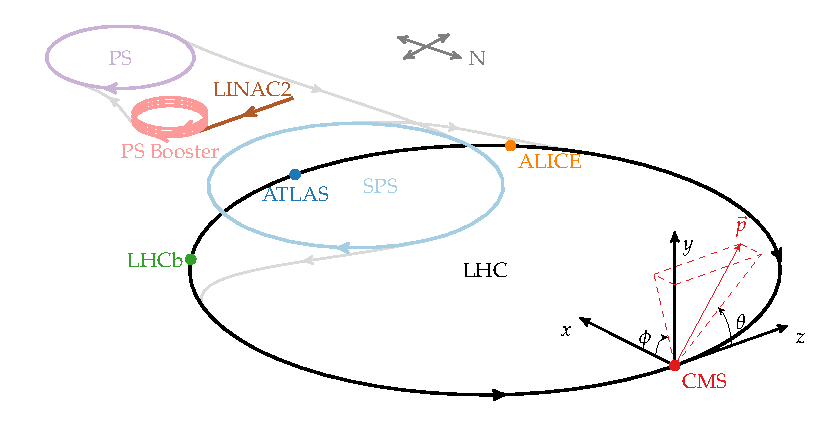
\includegraphics{diagrams/tikz/lhc_complex/lhc_complex.pdf}
    \caption{
        An isometric schematic view of the \LHC complex chain delivering
        proton-proton collisions at the four main detectors: \LHCb, \ATLAS,
        \ALICE and \CMS. The coordinate system used by the \CMS detector is
        shown in both cartesian and polar coordinates. The pseudorapidity
        $\eta$, defined as $-\ln(\tan(\theta/2))$, typically replaces the
        $\theta$ angle because of its convenient properties under Lorentz
        transformations. This diagram is not to scale and the relative
        positions of the rings are guides to the physical positions.
    }
    \label{fig:LHC-Complex}
\end{figure}


\subsection{\LHC Main Ring}

The main physics goals of the \LHC project was the discovery of the Higgs
boson, to observed new physics and rare \SM processes. The expected rate of a
particular process with a cross section $\xs$ at a integrated beam luminosity
$L$ is
%
\begin{equation}
    \mathcal{N} = L \xs \ .
\end{equation}
%
The event rate at the \LHC is directly controlled by the luminosity. For a
Gaussian distributed beam, the luminosity can be given in terms of beam
parameters as:
%
\begin{equation}
    \label{eq:beam-lumi}
    L = \frac{N_b^2 n_b\frev\relgamma}{4\pi\emitt\bstar} F\ ,
\end{equation}
%
where $N_b$ is the number of particles per bunch, $n_b$ is the number of
bunches per beam, \frev is the revolution frequency, \relgamma is the
relativistic gamma factor, \emitt is the normalised transverse beam emittance,
\bstar is the beta function at the collision point (related to the transverse
size of the beam) and $F$ is the geometric luminosity reduction factor due to
the crossing angle of each beam at the crossing point.

At the \LHC, the luminosity is maximised by tuning all parameters in
Eq.~\eqref{eq:beam-lumi}. This necessitated the use of proton beams
circulating in separate vacuum chambers and merging at insertion points to the
detectors. The beams nominally circulate in 2808 bunches with a spacing of
${\SI{25}{ns}}$ inside twin bore superconducting magnets --- two sets of coils
and beam channels within the same structure and cryostat --- achieving a peak
dipole field of ${\SI{8.33}{T}}$ to bend the beam. RF cavities apply the
potential gradient to accelerate the protons from ${\SI{450}{GeV}}$ to
${\SI{6.5}{TeV}}$. Quadrupole magnets focus the beam to suppress dispersion to
maintain the beam luminosity. Additional quadrupoles focus the beam as they
enter the collision sections and defocus as they exit  \cite{Bruning:782076}.


\section{Compact Muon Solenoid (\CMS) Experiment}

The conditions provided by the \LHC during 2016 data taking resulted in an
average number of collisions per bunch crossing of approximately 25, leading
to 1000 charged particles every ${\SI{25}{ns}}$ bunch crossing. The \CMS
detector \cite{Bayatian:922757} was designed to account for particle
multiplicities of this order by focusing on high-granularity subdetectors with
good time resolutions. This required a large number of detector channels and
millions of synchronised detector electronics, all with a high radiation
tolerance.

In addition to the conditions provided by the \LHC, the \CMS detector's design
was driven by four main physics requirements to achieve a broad range of
precision measurements and new physics searches, namely: searching for the
Higgs Boson, supersymmetric particles, new massive vector bosons, extra
dimensions; precision studies of the \SM; and heavy-ion physics. The physics
requirements are summarised as follows:

\begin{enumerate}
    \item \textbf{Muon identification:} ability to clearly identify muons up to
    $\aeta=2.4$ and dimuon mass resolutions of about $1\%$ for transverse
    momenta of \SI{100}{GeV}, with an unambiguous charge up momenta of
    \SI{1}{TeV}.
    \item \textbf{Charged particle reconstruction:} good momentum and
    reconstruction efficiency, particularly for the inner tracker, allowing
    for the identification of secondary vertices for the triggering and
    offline tagging $\tau$'s and $b$-jets. This requires a tracker component
    with a few cm of the interaction point.
    \item \textbf{Electromagnetic energy resolution:} measure the diphoton and
    dielectron mass with a resolution of $1\%$ for transverse momenta of
    \SI{100}{GeV} up to $\aeta=2.4$. In addition, efficiently reject backgrounds
    from \Ppizero decays into two photons and maintain prompt lepton isolation
    at high luminosities.
    \item \textbf{Transverse missing momentum and dijet mass resolution:} near
    complete reconstruction of the proton interaction to measure the
    transverse missing momentum. This requires a hermetic detector with hadron
    calorimeters extending up to $\aeta=5.0$ and fine component segmentation
    in the $\eta$-$\phi$ plane of less than $0.1\times 0.1$.
\end{enumerate}

The full design of the \CMS detector is shown in Fig.~\ref{fig:cms-full} which
achieves the requirements outlined above. The main distinguishing feature of
the \CMS detector is a ${\SI{3.8}{T}}$ superconducting solenoid magnet
enclosing the tracking and calorimetry subdetectors with and iron return yoke
to maintain a ${\SI{2}{T}}$ field outside the solenoid for the muon
subdetectors. All subdetectors are segmented into various regions in $\eta$
known as the barrel (covering the central $\eta$ range) and endcap (covering
up to $\aeta=3.0$, with a slight overlap with the barrel). The hadronic
calorimeter has an additional segment in the forward region, (covering
$3<\aeta<5$) as required for the missing momentum reconstruction. Further
subdetector dependent segmentation is done within the barrel, endcap and
forward regions; discussed in further detail in the following subsections.
This gives the \CMS detector a total length of ${\SI{21.6}{m}}$ and a diameter
of ${\SI{14.6}{m}}$ and weighing ${\SI{12500}{tons}}$.

\begin{figure}[htbp]
    \centering
    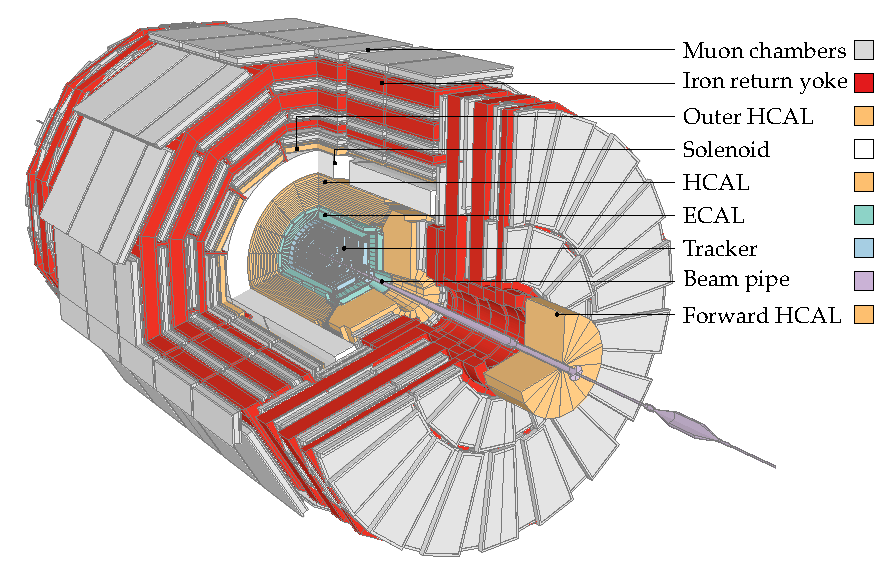
\includegraphics[]{diagrams/tikz/cms/annotated/cms_full.pdf}
    \caption{
        A schematic view of the \CMS detector and subdetectors with a section
        removed to view the internal components. Acronyms are explained in the
        text. The diagram was produced using the tools outlined in
        \cite{Sakuma:2013jqa}.
    }
    \label{fig:cms-full}
\end{figure}

\subsection{Silicon Tracker}

The inner most subdetector, the silicon tracker, measures the position of
charged particles from ionisation deposits (known as hits) across a
silicon-based reverse-biased p-n junction. A collection of hits is used to
reconstruct the curved trajectory, with a radius of curvature $r$, of the
particle with a charge $q$ within the magnetic field $B$ to determine the
momentum of the particle transverse to the field, \pt, given by:
%
\begin{equation}
    \pt = rqB\ .
\end{equation}
%
A collection of tracks may intersect at a common point leading to the
reconstruction of the primary interaction, pileup and secondary vertices.
These vertices are typically a few centimetres apart, therefore, the tracker
components are placed as near as ${\SI{4.4}{cm}}$ to the beam pipe.  The
silicon tracker, shown in Fig.~\ref{fig:cms-tracker}, consists of two main
components: pixels and strips. The pixels measure 3-dimensional positional
coordinates of hits for environments of high particle flux (up to 10 million
particles per second) near the beam. Pixel modules are aranged into three
layers placed in the barrel region (BPIX) at radii of ${\SI{4.4}{cm}}$,
${\SI{7.3}{cm}}$ and ${\SI{10.2}{cm}}$ with a length of ${\SI{53}{cm}}$,
centred on the z-axis. The pixel modules are staggered in the $\phi$-direction
to achieve an overlapping configuration. Two additional pixels layers are
placed in the both endcap regions (FPIX) with a turbine-like geometry with the
blades rotated by ${\SI{20}{\degree}}$ for overlapping blades. The overlap of
pixel modules ensures the charged particle passes through at least one module
in each layer. If two modules are hit the charge sharing between these modules
provides additional positional information on the hit leading to improved
position resolutions.

\begin{figure}[htbp]
    \centering
    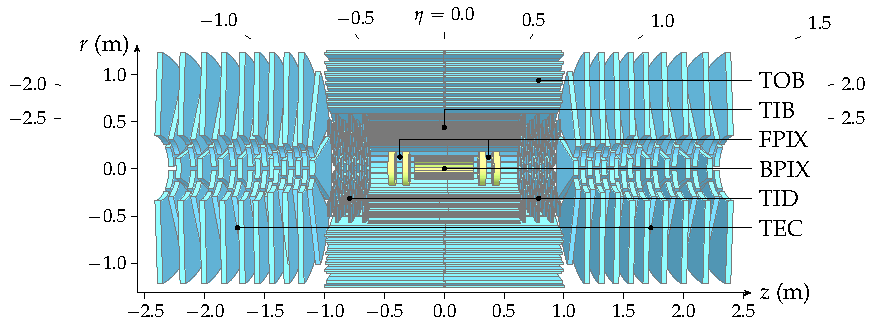
\includegraphics[]{diagrams/tikz/cms/annotated/cms_tracker.pdf}
    \caption{
        A cross-sectional view, in the $y$-$z$ plane, of the silicon tracker.
        The full tracker is shown in the upper part of the figure with a
        zoomed inset of the inner tracker in the central section and a further
        zoomed inset of the pixel tracker in the lowest part. The acronyms
        labelling various sub-components are defined in the text. The diagram
        was produced using the tools outlined in \cite{Sakuma:2013jqa}.
    }
    \label{fig:cms-tracker}
\end{figure}

Silicon strips are used further away from the beam pipe as the particle flux
reduces. Strips provide an accurate 2-dimensional position for hits, hence
layers are typically oriented in a stereo-configuration\footnote{A
stereo-configuration has layers rotated at an angle with respect to each other
to form a crosshatch pattern.} for the full 3-dimensional position. The
silicon strips are separated into an inner and outer component. The inner
component is further split by the barrel and endcap regions. The tracker inner
barrel (TIB) component consists of four layers positioned at a radius of
$20$--${\SI{55}{cm}}$ and covering ${|z|<\SI{65}{cm}}$ with cell sizes of
${\SI{10}{cm}\times\SI{80}{\micro m}}$. The first two layers use the
stereo-configuration with an angle of ${\SI{100}{mrad}}$. The tracker outer
barrel (TOB) component has six layers extending the coverage to
${|z|<\SI{110}{cm}}$ and ${\SI{55}{cm}<r<\SI{130}{cm}}$. Again the first two 
layers are place in a stereo-configuration with an angle of
${\SI{100}{mrad}}$. The inner endcap (TID) component provides coverage for the
gap between the TIB and TOB with three small disks oriented perpendicular to
the $z$-axis to avoid excessive shallow track crossing angles. The first two
disks have a stereo-configuration. The tracker outer endcap (TEC) consists of
nine disks extending into ${\SI{120}{cm}<|z|<\SI{280}{cm}}$ with
stereo-configuration for the first two  and the fifth disks
\cite{Borrello:687861}. The entirety of the silicon detector consists of 66
million pixels and 9.6 million silicon strips with near hermetic coverage up
to $\aeta=2.4$.

To process the data from the pixels and strips an on-detector chip processes
and buffers the analogue signal while waiting on a decision to accept or
reject the data (detailed in Sec.~\ref{sec:hardware-trigger}). Upon an accept
signal being received the data is transmitted over optical links to
off-detector chips for further processing, such as digitisation and data
formatting.


\subsection{\ECAL}

The \ECAL is a homogeneous calorimeter made of lead tungstate (\pbwo) crystals
designed to measure electromagnetic deposits (typically electrons and photons)
up to ${\aeta=3.0}$. The choice of lead tungstate scintillating crystals was
driven by their short radiation lengths, $X_0$ (${\SI{0.89}{cm}}$), and
Moliere radius \footnote{A radiation length is the distance travelled by a
particle through a material where, on average, the particle has lost $63.2\%$
of it's original energy. Similarly, the Moliere radius is the radius of a
cylinder which captures, on average, $90\%$ of the particle's shower,
transverse to the initial direction of travel.} (${\SI{2.2}{cm}}$) with fast
responses ($80\%$ of the light emitted is within ${\SI{25}{ns}}$) and have a
satisfactory level of radiation resistance. These properties allows a compact
design fully enclosed within the solenoid with sufficient containment of
electron and photon showers both laterally and along the length of the
crystals. The drawbacks of the crystal include low light yield
(${\SI{30}{photon/MeV}}$) requiring a coupling to photodetectors with
intrinsic gains operable in the magnetic field, and deterioration from
continuous irradiation monitored throughout.

The \ECAL is divided into the barrel section (EB) and the two endcap sections
enclosing the forward regions consisting of the endcap crystals (EE) and the
preshower (ES), diagrammatically shown in Fig.~\ref{fig:cms-ecal}. The EB has an inner
radius of ${\SI{129}{cm}}$ with the crystals titled at a ${\SI{3}{\degree}}$
angle in $\phi$ and $\eta$ with respect to the nominal vertex position to
avoid particles travelling fully between two crystals. The crystals cover a
$0.0174$ (${\SI{1}{\degree}}$) angle in $\phi$ and $\eta$ with the front face
cross-section of ${22\times\SI{22}{mm^{2}}}$ and a length of ${\SI{230}{mm}}$
corresponding to $25.8X_0$. A submodule consists of 5 pairs of crystals held
together by a thin-walled glass-fibre structure. The submodules are assembled
into groups of 40--50 including the readout electronics and thermal screen.
Four modules are placed side-by-side to create a supermodule that covers half
the length of the barrel and ${\SI{20}{\degree}}$ in $\phi$, two halves of 18
supermodules make the EB, covering a range of up to ${\aeta=1.479}$. The front
face of the EE are placed at ${|z|=\SI{314}{cm}}$ from the nominal vertex and
extends the \ECAL coverage in the range ${1.479<\aeta<3.0}$. Each endcap
consists of two dees --- semi-circular aluminium plates with structural
support units --- with crystals arranged in an $x$-$y$ grid of $5\times 5$
groups known as supercrystals. Partial supercrystals are placed on the inner
and outer boundaries of the EE. Each EE crystal has a frontal cross-section
of ${28.6\times\SI{28.6}{mm^{2}}}$ and a length of ${\SI{220}{mm}}$
(corresponding to $24.7X_0$). The ES is placed in front of the EE, covering
the range $1.653<\aeta<2.6$, and consists of two planes of silicon strip
detectors behind disks of lead absorbers at depths of $2X_0$ and $3X_0$,
respectively. The purpose of the ES is to initiate the electron or photon
showers with granular tracking to distinguish the individual photons from the
decay of ${\Ppizero\ra\gamma\gamma}$ for rejection and to provide directional
information on the electron or photon. A preshower placed in barrel was
rejected in favour of accommodating a larger tracker.

\begin{figure}[htbp]
    \centering
    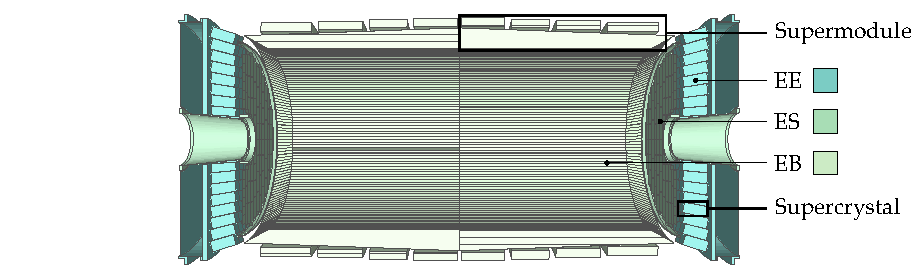
\includegraphics{diagrams/tikz/cms/annotated/cms_ecal.pdf}
    \caption{
        Front cross-sectional view of the \ECAL subdetector. Individual
        crystals are not shown, instead modules and supercrystals are
        displayed. The diagram was produced using the tools outlined in
        \cite{Sakuma:2013jqa}.
    }
    \label{fig:cms-ecal}
\end{figure}

The on-detector readout electronics for the \ECAL amplify and shape the signal
from the photodiodes and digitise at the bunch crossing rate of
${\SI{40}{MHz}}$. This data is buffered until an accept signal is received to
transfer the data to off-detector electronics for further processing. In
addition to this processing, the on-detector electronics run fast algorithms
on data from the ${5\times 5}$ clusters of crystals to aid in the accept
decision, detailed in Sec.~\ref{sec:hardware-trigger}.

The energy of a shower determined from photodiode signals is corrected to
reproduce the true energy of the particle initiating the shower. Several
factors result in the need for a correction factor, namely: an imperfect
clustering algorithm, energy loss from \brem, shower containment variations,
imperfections within the crystals, crystal-to-crystal variations, misalignment
of the crystals and limitations of the photodiodes. The reconstructed energy
of a shower, $E$, is given by
%
\begin{equation}
    E = G\mathcal{F}\sum_i c_i A_i\ ,
\end{equation}
%
where $G$ is the global absolute scale in converting GeV, determined from in
situ measurements of ${\PZ\ra\mu\mu\gamma}$. The function $\mathcal{F}$ is a
correction dependent on the type of particle; its position and momentum; and
the clustering algorithm used, determined from simulation validated by test
beam and in situ measurements of ${\PZ\ra ee}$ and ${\PZ\ra\mu\mu\gamma}$. The
product of $c_i$ --- the intercalibration coefficients obtained from
laboratory measurements, test beam precalibrations, comic ray measurements and
in situ ${\PW\ra e\nu}$ measurements, and ${\Ppizero\ra\gamma\gamma}$ and
${\eta\ra\gamma\gamma}$ mass reconstruction --- and $A_i$, the signal
amplitude, are summed over each clustered crystal labelled by $i$.

The corrected energy resolution of a supermodule is measured in a test beam by
fitting a gaussian function to the reconstructed energy distributions and
parameterised as
%
\begin{equation}
    \left(\frac{\sigma}{E}\right)^{2} = \left(\frac{S}{\sqrt{E}} \right)^{2}
    + \left( \frac{N}{E} \right)^{2} + C^2\ ,
\end{equation}
%
where $S$ is a stochastic tern, $N$ is a noise term and $C$ a constant term.
The total energy resolution ranges between {$1.50$--$0.35\%$} for
{$10$--$\SI{250}{GeV}$}, beyond which the constant term dominates.


\subsection{\HCAL}

The \HCAL is designed to provide full coverage of hadronic activity from a
proton-proton interaction, built from four distinct subdetectors, shown in
Fig.~\ref{fig:cms-hcal} found in the barrel (HB), endcaps (HE), beyond the
solenoid (HO) and far in the forward region (HF) \cite{Mans:1481837}. The HB
and HE subdetectors are sampling calorimeters, fully immersed within the
${\SI{3.8}{T}}$ field, with a brass absorber and plastic scintillator tiles in
a sampling ratio\footnote{The sampling ratio is the depth ratio of sampling to
absorbing elements.} of about $3:40$. The HB and HE are separated by a gap at
about $\SI{57}{\degree}$ designed to be non-projective with the interaction
point to avoid particles traversing an uninstrumented gap.

\begin{figure}[htbp]
    \centering
    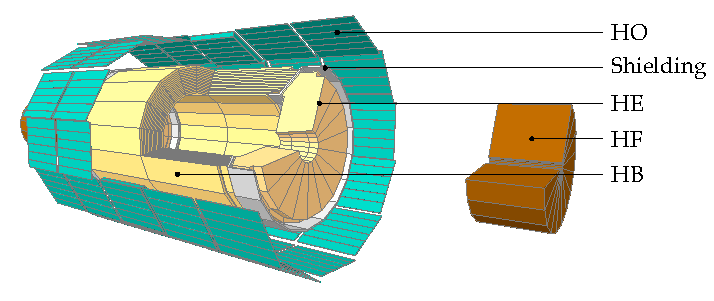
\includegraphics{diagrams/tikz/cms/annotated/cms_hcal.pdf}
    \caption{
        Front cross-sectional view of the four \HCAL subdetectors. The magnet
        between the HB and HO, along with the other subdetectors have been
        omitted. The HF is placed beyond the muon endcaps extending the
        coverage of the \HCAL in the forward region. The diagram was produced
        using the tools outlined in \cite{Sakuma:2013jqa}.
    }
    \label{fig:cms-hcal}
\end{figure}

The HB covers the central region up to $\aeta=1.4$ with a inner radius of
${\SI{1777}{mm}}$ and outer radius of ${\SI{2876.5}{mm}}$, made of two
half-barrels in $z$ of 18 identical wedges covering ${\SI{20}{\degree}}$ in
$\phi$ with further segmented into  ${\SI{5}{\degree}}$ sectors. The wedges
consist of towers: an alternating stack, parallel to the beam axis, of 17
active plastic scintillator tiles and brass plates, with the first and last
absorber replaced by steel for structural strength, forming a tower.
Constraints on the space  between the \ECAL and solenoid restricted the HB to
5.7 hadronic interaction lengths at ${\eta=0}$ and up to 9 at ${\eta=1.4}$,
necessitating the HO placed beyond the solenoid to improve the longitudinal
containment of hadronic showers. Scintillation photons are produced from the
interaction of hadronic showers with the active scintillation tile, collected
by wavelength shifting (WLS) fibres embedded within the plastic spliced to
clear fibres running along the tower. The optical signal is summed across the
depth of a tower in three groups: the first, the next 4 and the final 12
scintillator tiles (${\{1+4+12\}}$). The clear fibres are coupled to by
Silicon photomultiplers (SiPM). Full scintillator depth-segmentation would
allow hadronic shower discrimination, however, the segmentation is limited by
signal-to-noise, number of readout channels, power and cooling constraints.
Therefore, a balance of a three-depth configuration is in-place
\cite{Mans:1481837}.

The HE subdetector in the endcap provides coverage in the region
${1.3<\aeta<3.0}$, overlapping the HB for improved coverage across the
uninstrumented gap. The absorber-scintillator towers follow the same design as
the HB towers with wedges covering ${\SI{20}{\degree}}$ in $\phi$, segmented
to ${\SI{5}{\degree}}$ for towers in ${\aeta<1.74}$. The towers in
${\aeta>1.74}$ are instead segmented into ${\SI{10}{\degree}}$ to accommodate
the bending radius of the WLS fibres. The $\eta$ segmentation also increases
from ${0.087}$ for the towers at ${\aeta<1.74}$ to $0.09$--$0.35$ this $\eta$
range. The coarse azimuthal and polar segmentation allows for a finer depth
segmentation with configurations of four or five-depths in-place, grouped by
${\{1+2+3+5+7\}}$. The HE provides sufficient material interaction lengths
hence requires no outer calorimeter \cite{Mans:1481837}.

The HO consists of plastic scintillator tiles placed beyond the magnet to
catch energy leakage from the HB. Instead of brass, the solenoid and iron
return yoke act as the absorber extending the hadronic interaction lengths by
$2$--$3$. Two scintillator layers are placed at ${\eta=0}$, either side of a
${\SI{19.5}{cm}}$ thick piece of iron, where the interaction length of the HB
is the lowest. WLS fibres fed to SiPM detectors readout the signal from the
HO. The segmentation follows that of the muon system with ${\SI{30}{\degree}}$
wedges divides into ${\SI{5}{\degree}}$ sectors in $\phi$ to overlap with the
HB segmentation and five $\eta$ sectors up to ${\aeta=1.2}$. Partial plates
are placed around the cryogenics and power cables for the magnet.

High intensity radiation falls upon the HF, placed at ${|z|=\SI{11.2}{m}}$
downstream of the interaction point. Consequently, an alternative design of
steel absorbers embedded with radiation hard quartz fibres to produce
\cherenkov radiation from hadronic showers, detected by multi-anode
photomultiplier tubes \cite{Mans:1481837}. The steel absorbers are segmented
in $\phi$ by ${\SI{20}{\degree}}$ wedges subdivided into two
${\SI{10}{\degree}}$ sectors, apart from the two towers nearest to the beam
pipe which retain the ${\SI{20}{\degree}}$ segmentation. The steel absorber
towers are placed parallel to the beam axis with an $\eta$ segmentation of
approximately $0.175$, varying with $z$. The fibres also run parallel to the
beam axis placed ${\SI{5}{mm}}$ apart in an $x$--$y$ grid with alternating
long (full length of $10$ interaction lengths) and short (starting after $1.2$
interaction lengths). The two fibre lengths provide shower depth information
similarly to the depth segmentation in the HB and HE \cite{Abdullin2008HF}.

% Performance and calibrations?
%performance: Each subsystem has a laster and LED for monitoring and calibration. Since showers typically initiate in the ECAL the response and resolution of the CMS calo system depends on both the ECAL and HCAL. Corrections are determined from test beam studies. Resolution param by
%sigma/E = a/sqrt(E) oplus b
%From test beams of earlier HCAL designs: a = stochastic term and b constant term. a=0.847 +- 0.016, b=0.074 +- 0.008 for EB. EE is similar. HF has a=1.98 and b=0.09.
%
%calibrations: absolute energy scale, detector response and uniformity. Test beam of e, pi and mu. These are monitored with in situ measurements.
%performance: pions and electrons over 5-300 GeV. Low energy performance studied with muons. 


\subsection{Solenoid Magnet}

The muon identification requirement of the \CMS detector requires a large
bending power provided by the solenoid magnet with a field strength of
${\SI{3.8}{T}}$. Such a high field is obtained by a superconducting magnet,
shown in Fig.~\ref{fig:cms-magnet} maintained at operating temperatures by
superfluid helium cooling. To extend the bending power the return field is
focused by an iron return yoke spread throughout the muon chambers to about
${\SI{2}{T}}$.

\begin{figure}[htbp]
    \centering
    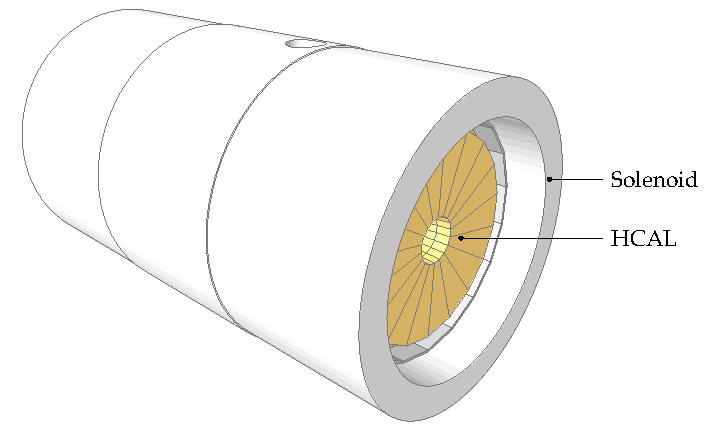
\includegraphics{diagrams/tikz/cms/annotated/cms_magnet.pdf}
    \caption{
        Isometric view of the solenoid and \HCAL with the muon chambers and
        HO removed. The diagram was produced using the tools outlined in
        \cite{Sakuma:2013jqa}.
    }
    \label{fig:cms-magnet}
\end{figure}


\subsection{Muon Chambers}

Muons from proton-proton collision, or secondary decays, travel through the
detector leaving tracks in the tracker and energy deposits in the calorimetry
system, however, most muons continue unscathed. The muon system is designed to
extend the 3-dimensional position measurements of these muons several metres
away from the interaction point. Three types of gaseous detectors are used
with the design driven by the large area to cover and different radiation
environments, particularly between the barrel and endcap.

The layout of the three gaseous detectors in the \CMS muon system is shown in
{Fig.~\ref{fig:cms-muon}}. In the barrel, anode wires centred in gas chambers,
known as a drift tubes (DT), collects the ionisation from passing charged
particles for 2-dimensional position measurements. DTs perform poorly in the
larger background and muon rate environment of the endcaps, hence cathode
stripe chambers (CSC) are in-place. A charged particle ionises the atoms of
the gas volume of a CSC with anode wires to collect the liberated electrons
and perpendicular copper cathode strips where a mirror charge is induced
allowing a full 3-dimensional position measurement. Resistive plate chambers
(RPC) accompany both the DTs and CSCs to provide fast responses with good
timing resolution at the cost of coarser positional resolution. The gas volume
within an RPC is ionised by charged particles with the liberated electrons
swept by an electric field induced from a large potential difference across
plastic tiles either side of the gas volume. The electrons are collected by
metal strips behind the plastic and the signal read out. The \CMS RPCs consist
of a double-gap separating ${\SI{2}{mm}}$ thick bakelite tiles by a
${\SI{2}{mm}}$ gas gap. 

\begin{figure}[htbp]
    \centering
    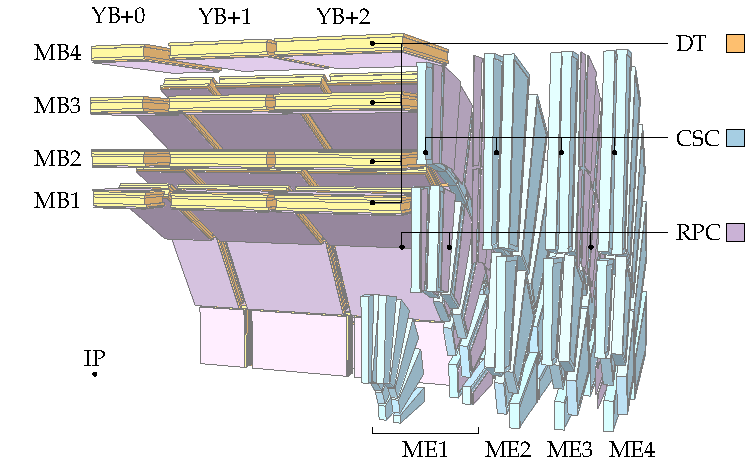
\includegraphics{diagrams/tikz/cms/annotated/cms_muon.pdf}
    \caption{
        Isometric view of the rear-top-right octant of the muon system,
        omitting the iron return yoke. The interaction point (IP) is shown in
        the lower left. The division of the muon system into stations (MB),
        wheels (YB) and disks (ME) are discussed in the text. The diagram was
        produced using the tools outlined in \cite{Sakuma:2013jqa}.
    }
    \label{fig:cms-muon}
\end{figure}

The muon barrel section (MB) cover ${\aeta<1.2}$ and consists of four concentric stations labelled MB1--MB4 position at about $4.0$, $4.9$, $5.9$ and ${\SI{7.0}{m}}$ away from the beam axis. Each station is subdivided into 12 sectors in $\phi$, with subsequent sectors overlapping to avoid uninstrumented gaps. Two partial sectors are placed around the magnet cryogenic lines and power cables. The MB is divided into five wheels along $\eta$ labelled $\mathrm{YB}-2$ to $\mathrm{YB}+2$. Stations MB1 and MB2 consist of two RPCs placed either side of a DT chamber whereas MB3 and MB4 have one RPC placed on the inside of a DT chamber. These DT chambers consist of four layers of drift tubes, known as a superlayer (SL). Two SLs have their anode oriented along the beam axis to measure the $r$-$\phi$ coordinates of muon tracks, $\mathrm{SL}_{\phi}$, and the third SL rotated by ${\SI{90}{\degree}}$ measures the $z$ coordinate (omitted in MB4), $\mathrm{SL}_{\theta}$. The SLs are separated by a honeycomb (HC) structure in the order: $\mathrm{SL}_{\phi}$, HC, $\mathrm{SL}_{\theta}$, $\mathrm{SL}_{\phi}$; where the final $\mathrm{SL}_{\phi}$ is omitted in MB4.

The muon endcaps (ME) enclose the solenoid both ends of the \CMS detector with
sufficient overlap with the barrel: $0.9<\aeta<2.4$. Both endcaps are divided
into four disks, labelled ME1--ME4, perpendicular to the beam axis, subdivided
into two concentric rings of 36 chambers (apart from ME2--ME4's innermost
rings with 18 chambers each). The chambers within a disk overlap to avoid
uninstrumented gaps. Each CSC is trapezoidal in shape with 6 gas gaps to
measure the $z$ position, cathode strips projecting radially outwards  to
measure the $\phi$ position and anode wires closely following the $\phi$
direction to measure the radial position from the beam axis. RPCs accompany
each CSC up to $\aeta=2.1$.

%- Readout
%- Calibrations
%- Alignment
    
\subsection{Hardware Trigger}\label{sec:hardware-trigger}

The ${\SI{40}{MHz}}$ bunch crossing frequency provided by the \LHC at 2016
luminosities yields on average 25 proton-proton interactions per crossing
leading to about 1 billion events per second. Storage capacities restrict full
detector archiving of about 100 crossings per second. Therefore, an online\footnote{Online refers to tasks or processes performed in real-time with strict timing constraints whilst data taking. Conversely, offline refers to processing after the storage of data without strict timing constraints.}
triggering system applies a rejection factor of the order of 1 in 10 thousand
with minimal impact to the broad physics program. This system is realised in
two-levels: the first level a hardware trigger (also known as the Level-1
trigger, \HWT) \cite{Bayatyan:706847,Tapper:1556311} with custom programmable
processors, and a second level a software trigger \cite{Sphicas:2002gg} using
general-purpose commercially available processors (discussed in
Sec.~\ref{sec:software-trigger}).

The detector data for each bunch crossing is held in on-detector buffers
whilst waiting on a decision from the \HWT to further process the crossing
with the software trigger. The \HWT processes up to 128 bunch crossings
simultaneously, allowing a total time of ${\SI{3.2}{\micro s}}$ on reaching a
decision. The allocated time includes data transit time to the electronics,
located in an adjacent cavern to the detector for radiation protection, which
reduces the total processing time to about ${\SI{1}{\micro s}}$. The \HWT is
sent a new bunch crossing to process every ${\SI{25}{ns}}$ and after the
allocated time a decision must be made, also every ${\SI{25}{ns}}$. These
restrictions prevent data fetching and result in most operations consisting of
simple arithmetic or querying memory in lookup tables\footnote{A lookup table
stores expensive computations in a pre-computed table for significant savings
in processing time and complexity.}. Furthermore, information from the tracker
and HO is omitted from the \HWT decision owing to their slow response. The
other subdetectors provide coarse information, to reduce processing time, and
are divided into the calorimeter and muon triggers with the candidates sent to
the global trigger for the final decision.

The \HWT decision is based on reconstruction of individual objects such as
photons, electrons, muons, jets, transverse energy sum or missing transverse
energy (\etmiss). The physics requirements can be summarised, with examples of
targeted physics, as follows:

\begin{enumerate}
    \item Triggering of events with a single lepton of ${\aeta<2.4}$ and
    ${\pt>\SI{40}{GeV}}$ with an efficiency above $95\%$ to target events with
    \PW decays.
    \item Dilepton triggers with the same kinematical requirements and an
    efficiency above $95\%$ to collect \PZ decays.
    \item Single photon and diphoton triggers with similar thresholds for
    processes involving a Higgs boson.
    \item \etmiss threshold about ${\SI{100}{GeV}}$ for sensitivity to new
    weakly interacting particles.
\end{enumerate}


\subsubsection{Calorimeter trigger}

\ECAL (EB and EE) and \HCAL (HB, HE and HF) signals are clustered into trigger
towers: ${5\times 5}$ arrays of crystals in the EB and EE; single physical
tower for the HE and HB up to ${\aeta=1.74}$ and twice the number of physical
towers in $\phi$ beyond this, whereby the energy of the physical tower is
divided equally between the trigger towers; and physical towers grouped into
pairs in $\phi$ and threes in $\eta$ for the HF. The transverse energy of each
trigger tower is determined by on-detector electronics and the result is sent
to the \HWT electronics along with flexible pass-fail information to, for
example, encode depth structure. This information is further processed with
each bunch crossing sent to one of ten processing nodes (with two redundant
nodes) to scan across the full ${\eta}$--${\phi}$ plane and identify physics
objects: jets, $\tau$s, electrons and photons; as well as calculating the
transverse energy sum and \etmiss. The processing nodes run concurrently with
a new bunch crossing occupying the first node upon completion of the previous
crossing. This is known as a time multiplexed system where the output must be
reassembled into the original bunch crossing order (de-multiplexed) for the
global trigger.


\subsubsection{Muon trigger}

The muon trigger system primarily consists of track finding from successive
chamber hits by a muon. This is divided into regional track finders using a
combination of the DTs and RPCs in the barrel (up to ${\aeta=0.8}$), CSCs and
DTs in the endcaps (from ${\aeta=1.25}$) and all three chambers in the overlap
region between the barrel and endcaps. Additionally, the system is tasked with
assigning hits to the correct bunch crossing, achieved by the high timing
precision of the RPCs and of the CSC's anode wire response. Timing is also
performed with the DTs, albeit with a poor resolution due to long drift times of
${\SI{400}{ns}}$. The tracks from these regional triggers is sent to the
global muon trigger to merge and remove duplicate muon candidates, along with
combining the isolation information from the calorimeter trigger, and finally
sorts the muons for the global trigger.


\subsubsection{Global trigger}

The trigger objects and variables received from the calorimeter and muon
triggers is collected at the global trigger for synchronisation and
correlation of relevant trigger candidates. The union of a set of requirements
on the trigger objects is determined and forms the basis of the \HWT decision.
However, evolving conditions and the collection of events from high
cross-sectional processes requires the global trigger to reject random events
to reduce the trigger rate. This process is known as prescaling and reduces
the trigger efficiency by the prescale factor: e.g. a prescale factor of 10
will accept 1 out of 10 events regardless of decision formed from the trigger
candidates resulting in a rate reduction of a factor of 10 and a drop
efficiency of $90\%$. After the prescaling is applied the \HWT decision is
communicated to the data buffers to discard or transmit the bunch crossing to
the software trigger.


\subsection{Software Trigger}\label{sec:software-trigger}

The software trigger (also known as the high-level trigger, \SWT) accepts the
full detector granularity and all subdetector information from the on-detector
readout. All bunch crossings filtered by the \HWT are distributed among
processing nodes in a processor farm, each node running a copy of the software
code to reconstruct and reject events. To meet the timing constraint, the \SWT
performs a partial reconstruction of the event at first, guided by the trigger
objects from the \HWT, gradually performing the full reconstruction until the
event fails the trigger criteria. Furthermore, the \SWT must be efficient at
selecting physics objects of interest and inclusive to avoid rejecting exotic
physics. Therefore, the \SWT reconstruction is closely aligned with offline
reconstruction (discussed in Chap.~\ref{chap:reconstruction}). However,
calibrations and other run conditions available for offline analysis cannot be
used. After accepting an event, the data is archived and made readily available
for further analysis by the computing grid.


\subsection{Worldwide \LHC Computing Grid (\WLCG)}

Despite the data reduction achieved by the \CMS trigger system, a vast amount
of data was accepted and requires prompt full reconstruction with possible
revisions in light of improved object reconstruction, calibrations or code
errors. Moreover, simulations of proton-proton collisions within the \SM and
possible \BSM physics, including a simulation of the detector, the trigger and
pileup with full reconstruction demands a significant amount of processing
power. To achieve this the \WLCG was established \cite{Bird:1695401}. The
\WLCG is a highly distributed computing cluster divided into tiers situated
at: the main \CERN site, national laboratories and Universities worldwide. The
computing  provides the resources required for data reconstruction and
simulations, and supports in the design, evaluation, construction and
calibration of the detector and future upgrades.


\section{Summary}

The \LHC provides proton-proton bunch crossings at a rate of ${\SI{40}{MHz}}$,
a centre-of-mass energy of ${\SI{13}{TeV}}$, and the \CMS detector centred on
one of these crossings. The \CMS detector is designed to detect and
reconstruct the position and momenta of outgoing particles from the collisions
whilst mitigating backgrounds such as noise and pileup, and optimising the
geometry and readout channels with modern technology. The main feature is a
${\SI{3.8}{T}}$ solenoid enclosing the silicon tracker and calorimetry with an
outer muon system. A two-level trigger system reduces the data output by
selecting events of interest for a manageable output rate for archiving.
The immense processing power required for further analysis of the data and
production of simulations is mediated by the \WLCG.
        \chapter{Event reconstruction}\label{chap:reconstruction}

%\chapterquote{}{}

\section{Introduction}

The apparent simplicity --- hits from ionising particles and energy deposits
from particle showers --- and the detector granularity of \CMS allows the
reconstruction and identification of muons, electrons and photons, and charged
and neutral hadrons. Instead of simply detecting, reconstructing and
identifying particles with their respective dedicated system an improvement is
made from correlating elements from all detector layers with an attempt to
distinguish each individual particle by a technique known as particle flow (PF).

The initial step in reconstruction, prior to the PF method, consists of
forming charged particle tracks from hits in the silicon tracker, tracks in
the muon chambers and calorimeter clusters from energy deposits in the
calorimetry system. The basic building blocks form the input into the PF
algorithm which attempts to link the various blocks into a coherent picture of
a particle candidate. For example, tracks are linked to an \ECAL deposit to
form an electron candidate with further linking to \ECAL deposits consistent
with Bremsstrahlung photons from the electron, which may undergo conversion
resulting in displaced electrons tracks also linked to the primary electron.
Furthermore, the reconstruction of all particles results in a simple \ptmiss
calculation from the negative vector sum of all particle momenta.

This chapter will describe in detail the process of tracking, clustering and
the PF method in the full reconstruction of a proton-proton interaction.


\section{Tracking}

Charged particles originating from the interaction point travel outward
through the magnetic field in helical trajectories. The hits in the silicon
tracker are reconstructed into the track by a fitting procedure known as the
combinatorial track finder. Hits are formed within the pixel tracker by
clustering deposits, above a certain threshold, in adjacent pixels. The
position of the hit for single pixel clusters is taken at the centre of the
pixel while multi-pixel clusters have a charge-weighted position, correcting
for the drift of electrons in the magnetic field. A more sophisticated,
albeit, computationally demanding method is used for the final track fit which
involves a $\chi^2$-fit of expected charge deposits from a large number of
simulated particles through the pixels to the observed charge deposit,
accounting for pixel deterioration. Strip tracker hits are formed from
clusters of adjacent strips with charge deposits exceeding a noise-level. The
hit position is determined from a charge-weighted average of the cluster,
correcting for the electron drift in the magnetic field and known
inefficiencies with the charge collection. All hits have an associated
uncertainty propagated to the track fitting procedure~\cite{Chatrchyan:1704291}.

The combinatorial track finder involves a series of Kalman filters (KF)
\cite{Kalman:1960} --- a recursive parameter estimator. A Kalman filter starts
with an initial state (a seed), typically from a guess or estimation,
and iterates across measurements updating the initial state parameters by
comparing the prediction to the observations. For track fitting, the fit is
performed to five parameters which describe points along a helical track, known
as the perigee parameterisation:
%
\begin{equation}
    \left( \frac{q}{\pt}, x_t, y_t, \theta_t, \phi_t \right)\ \,
\end{equation}
%
where $q/\pt$ is the ratio of the charge to track transverse momentum to give
the signed curvature scale of the trajectory. The parameters $x_t$ and $y_t$
are the distances from the interaction point to a point along the trajectory
in the $\vec{x}_t$ and $\vec{y}_t$ axis, shown in Fig.~\ref{fig:kf_parameters}
along with the definitions of the angles $\theta_t$ and $\phi_t$.

\begin{figure}
    \centering
    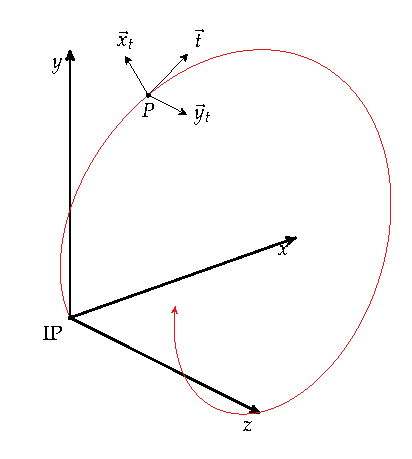
\includegraphics{diagrams/tikz/kf_parameters/kf_parameters.pdf}
    \caption{
        Diagram of a track (shown in red) from the interaction point (IP) with
        the conventional \CMS coordinate system as well as a local coordinate
        system along the trajectory, an example of which is shown at point $P$
        where $\vec{t}$ is the tangential vector, $\vec{x}_{t}$ is
        perpendicular to both the z-axis and $\vec{t}$ and $\vec{y}_{t}$ is
        the remaining vector to create a right-handed coordinate system. The
        angle between the $x$-axis and the projection of ${\vec{t}}$ onto the
        $x$-$y$ plane is $\phi_t$. Similarly, the angle between the $y$-axis
        and the projection of ${\vec{t}}$ onto the $y$-$z$ plane is $\theta_t$.
    }
    \label{fig:kf_parameters}
\end{figure}

The trajectory building with a Kalman filter starts with the seed generation
stage by combining a set of pixel hits, where the resolution is  a setthe
greatest and occupancy the lowest. Each iteration of the Kalman filter extends
to the next tracker layer where each hit candidate, within a $\chi^2$ window,
is kept to form independent track candidates. Fake tracks will typically have
a layer where no hits are within the window and can be dropped. Further checks
are performed on the consistency of hits with the \pt of the track and from
vertex constraints. Finally, a cleaning process assigns unique tracks to a
seed and vice versa. After determining the full set of tracks, the Kalman
filter procedure is repeated with the precise hit reconstruction, accounting
for inter-layer material and field inhomogeneities, with inflated
uncertainties to avoid biasing the initial result. Furthermore, the Kalman
filter is repeated, seeded by hits from the outermost layer iterating inwards.
The best fit tracks are taken from an average of the Kalman filter starting
from the inner layers and the reverse.

The trajectory building is performed ten times with different seeds to target
various classes of tracks with hits associated with candidate tracks removed
from subsequent iterations:
\begin{itemize}
    \item Prompt and high \pt tracks, and $b$-hadron decays are target by the
    first three iterations, seeded by three hits in the pixel detector with
    constraints on the track \pt and distance of nearest approach to the beam axis.
    \item The fourth and fifth iteration target tracks with one or two missing
    hits in the pixel detector as a result of particle interactions and
    decays, or detector inefficiencies. These are seeded by two pixel hits or
    a combination of three pixel and strips hits.
    \item The next two iterations are seeded by strip hits to target displaced tracks.
    \item The eighth iteration targets high \pt jets with merged constituent
    tracks, seeded by pairs of hits in the pixel and strips with the initial
    track compatible with a high energy calorimeter deposit.
    \item The final two iterations are designed to track muons missed by prior
    iterations by using information from the muon chambers to determine the seeds.
\end{itemize}
After all iterations are complete a full set of tracks within the tracker
volume are defined, known as inner tracks.


\subsection{Electron tracking}

Electron tracks may be missed by the combinatorial track finder as a result of
significant Bremsstrahlung and high energy photon emission. To recover these
tracks another fitting procedure is performed, based on a gaussian-sum filter
(GSF). The GSF method models hits by a weighted sum of gaussian distributions
for a more accurate representation of hits with sudden and substantial
radiative losses. The results of the expectation fit to the observed hits is
fed into a boosted decision tree\footnote{A boosted decision tree is a form of
supervised artificial learning with an output from a weighted linear sum of
many decision trees, determined by optimising a function of the truth and
prediction with a regularisation term to penalise tree depth.} (BDT) to
optimise electron track reconstruction efficiency while minimising fake
tracks. This procedure is also effective at tracking electron-positron pairs
from tracker converted photons.


\subsection{Muon tracking}\label{subsec:muon-tracking}

A track fitting procedure is performed with hits in the muon chambers to form
muon track candidates. Various quality muons are defined based on the inputs
and results of the track fitting:

\begin{itemize}
    \item \textbf{standalone muon:} track fitting seeds are formed of track
    segments from hits within the DT or CSC detectors. The fit itself uses
    hits within all muon chambers.
    \item \textbf{global muon:} a standalone muon track matched to an inner
    track.
    \item \textbf{tracker muon:} one muon segment matched to a unique inner
    track with requirements on the muon's momentum and its compatibility with
    an origin at the beam axis.
\end{itemize}


\section{Vertex reconstruction}\label{sec:vertex-reco}

The conditions provided by the \LHC during 2016 data-taking yielded on average
about 25 proton-proton interactions per bunch crossing. Since the triggering
system selects about 1 in 100 thousand crossing at most one of these
interaction points are of interest per event, known as the primary vertex. The
other vertices are classified as pileup which result in additional particles
leading to misreconstruction of the primary event. Therefore, the reconstruction
of these vertices is critical in mitigating the impact of pileup interactions,
particularly in determining the \ptmiss of the primary event.

The vertex reconstruction is performed by a fit to a selection of tracks. The
collection of tracks are selected by their track quality parameters
(sufficient number of hits and a satisfactory track fit $\chi^2$) and
consistency with the beam spot, a 3-dimensional profile of the luminous
region determined from an average over multiple bunch crossings. From these
track collections a set of vertex seeds are found by searching for convergence
points of multiple tracks \cite{Speer:927395}. These seeds initialises the
adaptive vertex fitter \cite{Fruhwirth:1027031}, a similar procedure to the
Kalman filter although all tracks are considered in turn weighted by the
compatibility of the track's nearest approach to the vertex seed. This is
followed by updating the vertex position from a method of least squares to the
weighted tracks. This procedure is iterated until convergence resulting in a
collection of vertex candidates. The primary vertex is selected from this
collection by the greatest $\sum \pt^2$ over all outgoing tracks
\cite{Sirunyan:2017ulk}.


\section{Calorimeter clustering}

A clustering algorithm groups energy deposits within the calorimeter towers to
encapsulate the whole extend of a particle shower, or multiple overlapping
showers. These clusters are sent to the PF algorithm to link the cluster with
a track, or multiple tracks. The clustering is performed separately in the
ECAL barrel and endcaps, HCAL barrel and endcaps, and the two preshower
layers. No clustering is performed in the HF since forward jets typically have
large momenta and hence collimated showers. Seeds initialise the clustering
and are identified as cells with an energy above a threshold and greater than
the nearest neighbouring cells. Topological clusters are formed by continually
merging neighbouring cells, with an energy twice the noise level, into the
cluster. Individual clusters within a topologial cluster are distinguished by
a gaussian-mixture model: a topological cluster in $M$ cells arise from $N$
gaussian energy deposits. The deposits are parameterised by the amplitude of
the $i$-enumerated gaussian, $A_i$; the position of the gaussian centre in
$\eta$-$\phi$, $\vec{\mu}_i$; and the width $\sigma$ of the gaussian, fixed to
values assigned for each calorimeter system. The initial values are taken from
the cell seeding the topological cluster and an expected energy fraction
measured in cell $j$ is determined from
%
\begin{equation}
    f_{ji} = \frac{A_i\exp\left(-(\vec{c}_i-\vec{\mu}_i)^2/(2\sigma^2)\right)}{\sum_{k=1}^{N}\exp\left(-(\vec{c}_j-\vec{\mu}_k)^2/(2\sigma^2)\right)} ,
\end{equation}
%
where $\vec{c}_i$ is the position of element $i$. The parameters are estimated
from an analytical maximum likelihood fit with
%
\begin{equation}
    A_i & = \sum_{j=1}^{M} f_{ji}E_j
\end{equation}
%
and
%
\begin{equation}
    \vec{\mu}_i & = \sum_{j=1}^{M} f_{ji}E_j\vec{c}_j\ ,
\end{equation}
%
where $E_j$ is the energy deposited in cell $j$. This fit is iterated until
convergence and the position and energy of the gaussian functions are taken as
the cluster parameters.

The energy of the clusters are calibrated to accurately reflect the true
energy deposited. The calibrations are applied independently to
electromagnetic and hadronic deposits, reflecting the difference in the
corresponding showers. Calibrations are determined from test beam data,
radioactive sources, cosmic ray measurements, in situ collision data and
simulated events.


\section{The particle flow algorithm}

The PF algorithm attempts to resolve all particles from the interaction point
by exploiting the high granularity of the \CMS detector. The algorithm must
deal with particle interactions within the detector leading to crooked tracks
(bent at a `kink') and secondary particles. Furthermore, to avoid a quadratic
computation with the number of particles only the nearest neighbouring PF
blocks in $\eta$-$\phi$ are considered as candidates in the linking algorithm.

The linking of inner tracks to muon tracks has been discussed in
{Sec.~\ref{subsec:muon-tracking}}. Calorimeter clusters are linked to inner
tracks by extrapolating the track to the \ECAL or \HCAL and a link formed if
these positions lie within a topological cluster's cells, allowing sufficient
margins to account for gaps in calorimeter coverage, shower profile
uncertainties and multiple scattering. A link distance quantifies the distance
between the extrapolated track position and the cluster position in
$\eta$-$\phi$ with the link of minimum distance kept. Bremsstrahlung photons
are linked to electron GSF tracks if tangents, at each tracker layer, to the
track are consistent with \ECAL clusters. A dedicated conversion finder
creates a link between two tracks and a photon if the track are compatible
with the characteristics of a photon conversion. Clusters are linked together
(preshower to \ECAL and \ECAL to \HCAL) if the more granular calorimeter
cluster is within the less granular calorimeter cluster, retaining the link
forming the minimum distance between the two clusters. Finally, tracks are
linked together through a common secondary vertex, attributed to
nuclear-interactions. These tracks must contain at least three tracks: one
incoming from the primary vertex and at least two outgoing, or at least three
outgoing. All links are formed and the subsequent part of the PF algorithm
recovers inefficiencies and removes fake particle candidates by targeting
particular particle classes, as follows.

    
\subsection{Muons}

Global muons are classified as isolated to avoid the misidentification of
charged hadrons, whereby the total energy in a cone of radius ${\Delta
R=\sqrt{\Delta\eta^2+\Delta\phi^2}=0.3}$ around the muon candidate must not
exceed $10\%$ of the muon \pt:
%
\begin{equation}
    I_{\mathrm{track,calo}} = \frac{1}{\pt}\Biggl(\bigg|\sum_{\substack{i\in \mathrm{tracks}\\\Delta R<0.3}} \vec{p}_{\mathrm{T},i}\bigg| + \sum_{\substack{j\in \mathrm{clusters}\\\Delta R<0.3}}E_{\mathrm{T}}\Biggr) < 0.1\ ,
\end{equation}
%
where $I_{\mathrm{track,calo}}$ is known as the track-calorimeter isolation,
$i$ sums the transverse momenta of all tracks within $\Delta R=0.3$ and $j$
sums the transverse energies of all clusters within $\Delta R=0.3$.
Non-isolated muons are also identified without the isolation requirement,
however, inner tracks must match at least three track segments in the muon
detectors or calorimeter clusters compatible with the muon hypothesis to avoid
high \pt charged hardon misidentification.

The \pt of PF muon candidates is reconstructed from the tracker for
${\pt<\SI{200}{GeV}}$, otherwise the \pt is taken from the track fit resulting
in the lowest $\chi^2$ from the following combinations of information: tracker
only, tracker and the first muon detector plane, global muons, and global muons
without high occupancy muon detector planes. After all PF muon candidates are
identified and reconstructed the associated PF blocks are removed from further
candidate identification. Note that under certain conditions charged hadrons
may later be revised as muons.


\subsection{Electrons and isolated photons}

Electron and isolated photon reconstruction must collect and associate
Bremsstrahlung photons and electrons from photon conversions to accurately
measure the true energy of these particles. These secondary particles are
associated to a seed candidate: an \ECAL supercluster above a transverse
energy threshold of ${\SI{10}{GeV}}$ with no GSF track link for photons, or
GSF tracks associated to \ECAL clusters with fewer than three additional
linked tracks. Both classes of candidates must not have \HCAL clusters within
${\Delta R=0.15}$ of the candidate with an energy deposit exceeding $10\%$ of
the supercluster energy. The assigned energy of the candidate is determined
from the sum of all energy deposits linked to the seed, this includes
Bremsstrahlung photons at tangents to GSF tracks at tracker layers and GSF
tracks found by the conversion finder. This energy is calibrated and taken as
the final energy for isolated photon candidates. Electron candidate's energy
is determined from a combination of the calibrated \ECAL energy and GSF track
momentum.

To further reduce misreconstruction the candidates must pass additional
criteria. A BDT is trained separately for the barrel and endcaps, and for
isolated and non-isolated electrons with a requirement placed on the output
determined by the following input features: energy radiated from the GSF
track, distance between the GSF track extrapolation and the \ECAL seeding
cluster, ratio of the \HCAL to \ECAL energy, KF and GSF track $\chi^2$ and the
number of hits in the tracker. Photons, on the other hand, are required to be
isolated from other tracks, calorimeter clusters and have \HCAL to \ECAL
energy ratios consistent with typical photon showers.

Finally, as with muons, the PF blocks associated with the electron and
isolated photon candidates are removed from further processing.


\subsection{Hadrons and non-isolated photons}

The remnants of jet fragmentation and hadronisation with the subsequent decay
of heavy hadrons include: charged hadrons such as $\Ppipm$, $\Pkpm$ and
protons; neutral hadrons such as $\Pklzero$ and neturons; non-isolated photons
typically from $\Ppizero$ decays; and rarely additional muons from early
charged hadron decays. Discrimination of hadrons, other than charged and
neutral, is difficult with high misidentification rates, therefore, the PF
algorithm makes no attempt at this distinction.

From the remaining PF blocks, all \ECAL clusters within the tracker acceptance
(${\aeta<2.4}$) with no linked tracks are considered as photons. Similarly,
\HCAL clusters with the same acceptance with no linked tracks are treated as
neutral hadrons. This assumption holds well within the tracker acceptance where
charged and neutral hadrons are distinguishable and $25\%$ of the jet's energy
is deposited in the \ECAL as photons while only $3\%$ as neutral hadrons
($1\%$ for $\tau$-lepton decays as a result of Cabibbo-suppression). However,
beyond ${\aeta=2.4}$ up to the \ECAL acceptance (${\aeta<3.0}$) the precedence
to photons leads to a high misidentification rate of charged and neutral
hadrons, which can account for $25\%$ of the jet's energy deposited in the
\ECAL. Instead, \ECAL clusters linked to \HCAL clusters are assigned as hadron
showers with an unknown charge, while \ECAL clusters without this link are
considered photons. Beyond ${\aeta=3.0}$, within the HF, electromagnetic and
hadronic activity are identified by exploiting depth information and lateral
shower profiles by comparing $3\times 3$ to $5\times 5$ clusters.

Misidentification and misreconstruction may leave inconsistencies in the
calibrated calorimetric energy and tracker momenta for charged hadrons. These
are dealt by reassigning the identification or refining the reconstruction,
since the excess infers the presence of photons or neutral hadrons. If the
calibrated cluster energy $E_T$ is in excess, by $\delta_T$, of the sum of
linked track momenta, $|\sum \vec{p}_T|$, where ${\SI{500}{MeV}<\delta_T<E_T}$
then $\delta_T$ is attributed to a photon. If $\delta_T>E_T$, the $E_T$
deposit is revised as a photon and $\delta_T$ is assigned to a neutral hadron.
If the excess is small but inconsistent with the energy resolution
$\sigma(E_T)$, ${\sigma(E_T)<\delta_T<\SI{500}{MeV}}$, a $\chi^2$ fit to the
tracker and calorimeter information is performed to refine the energy of the
charged hadron. Finally, in the rare case where the track momenta are in
excess of $E_T$, i.e. $\delta_T<0$, a relaxed search for muon candidates is
performed. Any remaining excess is associated to misreconstructed tracks with
a momentum resolution greater than ${\SI{1}{GeV}}$. The leading\footnote{Leading refers to the candidate in a collection with the largest \pt.} misreconstructed track candidate is repeatedly removed until no excess or no
candidates remain.

Displaced tracks within the tracker volume predominantly from nuclear
interactions are yet to be identified. These involve secondary
charged particle tracks linked to a secondary vertex. The charged particles
are replaced by a single charged hadron, conserving energy and momentum, with
a mass of a charged pion. If a primary charged particle track exists, with a
well-defined momentum, then any deficit in the outgoing energy is attributed
to undetected secondary particles and the energy of the primary charged
hadron is updated to account for these particles.


\subsection{Jets}

The fragmentation and hadronisation of outgoing quarks form a cone of hadrons
known as a jet. The anti-\kt algorithm \cite{Cacciari:2008gp,Cacciari2012}
discussed in Sec.~\ref{sec:theory} clusters PF candidates into cones of
radius $R=0.4$ in the $\eta$-$\phi$ plane.  The minimum clustering threshold
is set to $\SI{15}{GeV}$, below which jets are unreliable at mirroring the
underlying physics. Seeding jets by PF candidates improves the energy
resolution by complimentary tracker measurements for charged hadrons affected
by the poorer hadron calorimeter resolution. However, as with any other jet
seed, neutrinos from hadron decays within  the jet are not accountable.


\subsection{Missing transverse momentum}

The PF method allows a simple calculation of the uncorrected (or raw) \ptmiss
from:
%
\begin{equation}
    \vec{p}_{\mathrm{T,raw}}^{\mathrm{miss}} = - \sum_{i} \vec{p}_{\mathrm{T},i}\ ,
\end{equation}
%
where $i$ sums over the PF candidates. However, residual misidentification and
misreconstruction can lead to a large \ptmiss similar to new physics
processes. To control the artificially large \ptmiss all particles with a
significant correlation with the direction and magnitude of the \ptmiss are
selected. The particles are typically high \pt muons and their identification
and reconstruction revised as follows:
%
\begin{itemize}
    \item \textbf{Genuine cosmic ray muons} in coincidence with an \LHC beam
    crossing, positioned further than ${\SI{1}{cm}}$ from the beam axis, are
    removed from the PF candidate collection if this leads to a reduction in
    the \ptmiss of at least a half. Semi-leptonic decays of $b$-hadrons are
    protected as their removal would increase the \ptmiss.
    \item \textbf{Severely misreconstructed muon momentum} as a result of
    wrong track association, steel yoke interactions, in-flight decay or
    significant synchrotron radiation. Here, the reconstruction of muons with
    ${\pt>\SI{20}{GeV}}$ is reviewed and the \pt updated if it leads to a
    reduction in the \ptmiss by at least a half.
    \item \textbf{Particles misidentified as muons} typically from
    charged-hadronic punch-through into the muon systems. In this case, neutral
    hadron deposits within the calorimeters are wrongfully included as
    independent particles leading to a double-counting of the charged hadron
    as a muon and a neutral hadron. Provided that the \ptmiss is reduced by a
    half and the muon momentum and neutral hadron energies are larger than
    ${\SI{100}{GeV}}$, then the neutral hadron is removed and the muon is
    revised as a charged hadron.
    \item \textbf{Muon and neutral hadron overlap} with similar energies which
    are misidentified as a charged hadron. The charged hadron is converted
    into a muon and a neutral hadron if the associated \ptmiss is reduced by a
    half.
\end{itemize}
%
After these revisions the \ptmiss is updated and the approach validated with
in situ measurements and studies in simulated events which show minimal impact
on processes with real \ptmiss, such as the pair-production of $t\bar{t}$.


\section{Summary}

The \CMS software reconstruction incorporates the whole detector, correlating
detector elements to improve particle identification and reconstruction with an
attempt to reconstruct all detectable particles in a technique known as
particle flow. The PF algorithm starts from two basic building blocks: tracks
and clusters. Tracks are formed from a series of Kalman filters applied to
hits: charge deposits within the tracks. An alternative GSF track finder
attempts to reconstruct the tracks of electrons subject to radiative losses.
Vertex reconstruction is performed from a fit to high-quality track candidates
consistent with the beam spot and the primary interaction point identified as
the vertex with the greatest $\sum \pt^2$ over outgoing tracks. On the other
hand, clusters are formed from energy deposits within calorimeter cells,
grouped and refined by a gaussian-mixture model. 

The PF algorithm links the building blocks (tracks and clusters) to form a
coherent picture of each individual particle with complementary measurements
from the various subdetectors. Muon candidates have links between inner and
muon chamber tracks. Electron and isolated photon candidates are formed from
\ECAL clusters, linked to GSF tracks for electrons, with further linking to
clusters consistent with Bremsstrahlung photons or GSF tracks compatible with
photon conversions. Hadrons and non-isolated photons have possible links
between tracks, \HCAL and \ECAL clusters. Further refinement is performed on
irregular candidates. After all PF candidates are determined jets are
clustered from all candidates with the anti-\kt algorithm and the \ptmiss
determined from a negative sum over all candidate $\vec{p}_{\mathrm{T}}$
with possible identification revisions to avoid large spurious
\ptmiss.
        \chapter{Event Selection and Categorisation}
\label{chap:analysis}

%\chapterquote{}{}
% \cite{Alwall:2014hca}.

\section{Introduction}

The measurement of the \IZinv width requires the collection of \IZvvj signal events with the key signature of jets recoiling against an invisible system, also known as \metplusjets. The \IDYllj process is used as a reference to extract the invisible width, under the assumption of a purely \SM \IZll interaction. In addition, samples of \IWlvj provide a data-driven estimate of large backgrounds with a similar signature to the signal. A combination of the large QCD multijet cross-section and inherent jet misreconstruction leads to additional backgrounds and the need of a sideband\footnote{A sideband is an independent set of events to a region obtained by inverting or somehow altering a requirement which defined the original region.} enriched with QCD multijet events for a data-driven estimate of this background.

This chapters details the process of data collection and reduction to target specific processes in various categories required for this analysis. Included is the detail of particle identification refinement from the PF algorithm results for an improved signal acceptance whilst maintaining a high background rejection.

\section{Samples}

\subsection{Data collection}

Detector measurements associated to a proton-proton bunch crossing are stored by various sets of \SWT requirements, known as \SWT paths. The dataset under consideration was collected during 2016 with proton-proton collisions at a centre-of-mass energy of ${\SI{13}{TeV}}$. Issues during detector live-time, such as problems with a particular subdetector or beam conditions, requires the rejection of problematic data resulting in a dataset with an integrated luminosity of ${\SI{35.9}{fb^{-1}}}$.

The relevant process can be classified into events with missing transverse momentum or more than one lepton. Events with a significant missing transverse momentum are selected by the \SWT paths requiring two conditions or a third to be satisfied. The first is
%
\begin{equation}\label{eq:hlt_met_trig_selection1}
    \ptmissnomu = \bigg| -\sum_{i\not\in\mathrm{muons}} \vec{p}_{\mathrm{T}} \bigg| \ge \ptmissthresh\ ,
\end{equation}
%
where the sum is over all PF candidates apart from muons and \ptmissthresh is a particular threshold. The muons act as invisible particles for \ptmissnomu hence this collects \IZvv, \IWmv and \IDYmm events. The second condition is
%
\begin{equation}
    p_{\mathrm{T,had}}^{\mathrm{miss}} = \bigg| -\sum_{i\in\mathrm{jets}} \vec{p}_{\mathrm{T}} \bigg| \ge \ptmissthresh\ ,
\end{equation}
%
summed over all PF jets passing the tight jet identification selection with ${\pt>\SI{20}{GeV}}$ and no muon candidates. This selection is similar to Eq.~\ref{eq:hlt_met_trig_selection1}, however, the combination of both maintains a trigger rate for lower \ptmissthresh  thresholds by removing events with inconsistent visible (excluding muons) and hadronic recoils, primarily due to misreconstructed soft (${\pt<\SI{20}{GeV}}$) hadronic activity. The threshold \ptmissthresh varies from {$90$--$\SI{120}{GeV}$} depending on the \LHC beam conditions to avoid prescaling. The third condition recovers small inefficiencies by applying the selection
%
\begin{equation}
    \ptmiss = \bigg| -\sum_{i\in\mathrm{PF}} \vec{p}_{\mathrm{T}} \bigg| \ge \SI{170}{GeV}\ ,
\end{equation}
%
summed over all PF candidates, with various beam halo or \HCAL noise cleaning requirements (discussed in Sec.~\ref{sec:baseline-selection}) to maintain this threshold as beam conditions change.

A complementary trigger path collects events with at least one muon rather than the momentum imbalance of an event. Events pass the trigger requirement if there exists a global or tracker muon with ${\pt>\SI{24}{GeV}}$ which is isolated from other activity (total energy within a cone of $\Delta R=0.3$ is below $9\%$ relative to the muon \pt). To collect events with at least one electron an alternative trigger path is used with the requirement of at least one GSF electron passing a tight identification selection and a ${\pt>\SI{27}{GeV}}$. Both lepton trigger thresholds are driven by a goal to maintain data collection efficiency and control trigger rates.


\subsection{Simulation}

A vast array of simulated proton-proton collisions attempt to fully replicate the events selected as signal candidates, including backgrounds with similar experimental signatures to the signal. Vector boson production; namely \IZvv, \IWlv, \IDYll and prompt photon; in association with jets, \IVj, are produced with the matrix element (ME) event generator \MADGRAPH \cite{Frederix:2018nkq} with restricted boson decays and Feynman diagrams up to $\mathcal{O}(\alpha^2\alpha_s^2)$, hereby known as next-to-leading order (NLO) in the strong coupling constant. The production is split into boson \pt regions to populate the low cross-section high-\pt regions. These generated events are coupled to the \PYTHIA package \cite{Sjostrand:2014zea} to mediate the parton showering (PS), hadronisation and particle decays with the \CUET underlying event description \cite{Khachatryan:2015pea}. Double-counting of jet multiplicity final states with the ME and PS is removed by the FXFX \cite{Frederix:2012ps} matching and merging technique. Another set of processes similar to \IDYll are generated where, in turn, the \PZ and \Pgstar interactions are turned off to model the \PZ, \Pgstar and interference terms of the \IDYll process. Furthermore, the processes involving a \Pgstar have an invariant mass cut-off below ${\SI{50}{GeV}}$ to avoid the large cross-section away from the \PZ peak.

Minor background processes include the pure QCD interactions between partons forming a multijet final state with jet misreconstruction leading to spurious \ptmiss, faking the signal signature. The QCD multijet process is produced at leading order (LO) accuracy in the strong coupling constant by the \PYTHIA package, split by the interaction scale $Q^2$ to populate the low cross-section regions. Top production leads to real \ptmiss with zero, one or two leptons in the final state with the pair production, \Ittj, produced using a similar technique as the \IVj processes, albeit inclusive in \pt, and single top production --- via the $s$-channel, $t$-channel or associated \PW production --- are produced at NLO by a various combination of the \MADGRAPH, \MADSPIN \cite{Artoisenet:2012st}, \PYTHIA and \POWHEG \cite{Alioli:2010xd,Alioli:2009je,Re:2010bp} packages. Diboson processes (combination of \PZ, \PW and prompt \Pgamma from the hard scatter) may have a similar signature to the signal for particular decays, or particles beyond the detector's acceptance or misidentified. Combinations of \MADGRAPH, \MADSPIN, \PYTHIA and \POWHEG are used to generate the diboson process at NLO. Finally, vector boson scattering (VBS) involves the production of a vector boson (\PW or \PZ) from $\PV\PV$ scattering, in association with two jets, hence has a signature similar to the \IVj processes. The VBS sample is produced at LO accuracy by the \MADGRAPH package coupled to \PYTHIA, with the boson decay restricted to charged leptons or neutrinos. An overlap between the phase-space of the diboson and VBS samples is removed by an ad hoc requirement of one generated boson from the hard scatter for VBS.

All samples are generated with \NNPDF \cite{Ball:2014uwa} LO and NLO parton distribution functions, where the LO and NLO generators are used. After the relevant process has been generated the full detector response to such an interaction, along with pileup vertices, is simulated with the \GEANT \cite{AGOSTINELLI2003250} package.


\section{Physics objects}

Analysis specific physics objects are derived from PF candidates to refine and target the selection towards the key signature. These include muons; electrons; photons; jets with tagging as hadronic $\tau$-lepton decays or $b$-hadrons; and the global event descriptor $\ptmiss$, redefined in terms of the recoil parameter.

\subsection{Muons}

The analysis definition of a muon is split into two categories: veto and selection muons. The selection defining these categories is shown in Tab.~\ref{tab:muon-selection}. Muons from in flight hadron decays are suppressed by a requirement on the particle-based isolation $I_{\Delta\beta}$ with a pileup mitigation term, known as the $\Delta\beta$ correction
%
\begin{equation}
    I_{\Delta\beta} = \frac{1}{\pt}\left| \sum_{i\in\mathrm{ch}}\vec{p}_{\mathrm{T},i} + \max\left( 0, \sum_{i\in\mathrm{nh}}\vec{p}_{\mathrm{T},i} + \sum_{i\in\gamma}\vec{p}_{\mathrm{T},i} - \frac{1}{2}\sum_{i\in\mathrm{PU\ ch}}\vec{p}_{\mathrm{T},i} \right)\right|\ ,
\end{equation}
%
for a muon with transverse momentum \pt; charged hadrons (ch), neutral hadrons (nh) and photons (\Pgamma) from the primary vertex in a cone of $\Delta R=0.4$ around the muon; and charged hadrons from pileup vertices (PU ch) also within this cone. This correction mitigates the contribution from neutral hadrons from pileup vertices by subtracting the momentum of charged hadrons from these vertices, with a factor of a half to account for the average charged-to-neutral particle ratio in the isospin limit. Additional selection is placed on the quality of selection muon tracks, including the impact parameter with the primary vertex split by the transverse, $d_{xy}$, and longitudinal, $d_{z}$, components.

\begin{table}[htb]
    \centering
    \begin{tabular}{lcc}
        \hline\hline
        & Veto & Selection \\
        \hline
        Muon seed & Global or tracker & Global \\
        PF muon & True & True \\
        Track fit normalised $\chi^2$ & - & $<10$ \\
        Number of matched stations & - & $>1$ \\
        Number of muon chamber hits & - & $>0$ \\
        $d_{xy}$ (cm) & - & $<0.2$ \\
        $d_{z}$ (cm) & - & $<0.5$ \\
        Pixel hits & - & $>0$ \\
        Tracker layer hits & - & $>5$ \\
        $I_{\Delta\beta}$ & $<0.25$ & $<0.15$ \\
        \pt (GeV) & $>10$ & $>30$ \\
        \aeta & $<2.5$ & $<2.4$ \\
        \hline\hline
    \end{tabular}
    \caption[Requirements placed on muons.]{
        Requirements for muons passing the veto and selection identification.  Most track quality criteria are omitted for veto muons to retain a high efficiency at the loss of fake muon rejection \cite{CMS-DP-2017-007}. The \pt requirement on selection muons is driven by trigger requirements for the single muon triggers used for the \ptmiss trigger efficiency measurements.
    }
    \label{tab:muon-selection}
\end{table}

%The veto criteria are highly efficient at selecting prompt muons and muons from heavy and light quark decays, while the selection criteria 

\subsection{Electrons}

Similar to muons, the electrons are classified as veto or selection based on criteria detailed in Tab.~\ref{tab:electron-selection}. The first requirements primarily reduce fake electrons from jets with criteria on $\sieiefbf$, the extent of the shower along the \ECAL crystals in the $\eta$ direction within a $5\times 5$ crystal cluster, typically smaller for electrons and photons than hadronic showers; and $E_{\mathrm{\HCAL}}/E_{\mathrm{\ECAL}}$, the ratio of the energy deposited in \HCAL towers located behind the \ECAL cluster to the \ECAL cluster energy, significantly smaller for electron and photons compared to jets. Subsequent requirements check the consistency of the GSF track with the \ECAL cluster, namely $|\Delta\eta_{\mathrm{In}}|$, the difference in $\eta$ of the energy-weighted supercluster centre and the GSF track extrapolated to the \ECAL; $|\Delta\phi_{\mathrm{In}}|$, similarly defined in the $\phi$ direction; $|(1/E_{\mathrm{\ECAL}} - 1/p_{\mathrm{T,track}})|$; and the impact parameters $d_{xy}$ and $d_{z}$. The conversion veto rejects electrons with tracks consistent with photon conversions identified by the conversion finder. The isolation, $I_{\mathrm{EA}}$, requirement on electrons reduces contamination from in flight hadron decays, with a pileup mitigation technique known as effective area:
%
\begin{equation}
    I_{\mathrm{EA}} = \frac{1}{\pt} \left| \sum_{i\in\mathrm{ch}} \vec{p}_{\mathrm{T},i} + \max\left(0, \sum_{i\in\mathrm{nh}}\vec{p}_{\mathrm{T},i} + \sum_{i\in\Pgamma}\vec{p}_{\mathrm{T},i} - \rho A_{\mathrm{eff}}\right) \right|\ ,
\end{equation}
%
which is similar to $I_{\Delta\beta}$, however, the subtracted quantity is the product of the energy density $\rho$, defined by the total energy of the event per unit area in $\eta$--$\phi$, of the event with the ($\eta$-dependent) effective area of the electron, a pre-computed average over multiple events.

\begin{table}[htb]
    \centering
    \begin{tabular}{lcccc}
        \hline\hline
        & \multicolumn{2}{c}{Veto} & \multicolumn{2}{c}{Selection} \\
        & Barrel & Endcaps & Barrel & Endcaps \\
        \hline
        GSF track & \multicolumn{4}{c}{True} \\
        \sieiefbf & 0.011 & 0.0314 & 0.00998 & 0.0292 \\
        $E_{\mathrm{\HCAL}}/E_{\mathrm{\ECAL}}$ & 0.298 & 0.101 & 0.0414 & 0.0641 \\
        $|\Delta\eta_{\mathrm{In}}|$ & 0.00477 & 0.00868 & 0.00308 & 0.00605 \\
        $|\Delta\phi_{\mathrm{In}}|$ & 0.222 & 0.213 & 0.0816 & 0.0394 \\
        $|(1/E_{\mathrm{\ECAL}} - 1/p_{\mathrm{T,trk}})|$ (1/GeV) & 0.241 & 0.14 & 0.0129 & 0.126 \\
        $d_{xy}$ (cm) & 0.05 & 0.1 & 0.05 & 0.1 \\
        $d_{z}$ (cm) & 0.1 & 0.2 & 0.1 & 0.2 \\
        Missing tracker hits & \multicolumn{4}{c}{2} \\
        Conversion veto & \multicolumn{4}{c}{True} \\
        $I_{\mathrm{EA}}$ & 0.0994 & 0.107 & 0.0588 & 0.0571 \\
        \pt (GeV) & \multicolumn{2}{c}{$>10$} & \multicolumn{2}{c}{$>30$} \\ 
        \hline\hline
    \end{tabular}
    \caption[Criteria to select and veto electrons.]{
        Criteria for the electrons identified as veto or selection for the analysis. These values tuned to obtain a pre-defined efficiency and background rejection. All parameters must be less than the value unless stated otherwise. The criteria are split by barrel and endcap regions to retain similar electron identification efficiency in both \cite{CMS-DP-2017-004}.
    }
    \label{tab:electron-selection}
\end{table}

\subsection{Photons}

The selection for photons is closely aligned with electrons, although with a single veto category and without tracker based requirements and an explicit rejection of candidates linked to tracks. Furthermore, the isolated requirements are split by particle candidates: charged hadrons, neutral hadrons and photons; with a \pt-dependence to remain efficient across a broad range of momenta. The selection is detailed in Tab.~\ref{tab:photon-selection}.

\begin{table}[htb]
    \centering
    \begin{tabular}{lcc}
        \hline\hline
        & Barrel & Endcaps \\
        \hline
        Linked track & False & False \\
        \sieiefbf & 0.01031 & 0.03013 \\
        $E_{\mathrm{\HCAL}}/E_{\mathrm{\ECAL}}$ & 0.0597 & 0.0481 \\
        $I_{\mathrm{ch}}$ & $1.295/\pt$ & $1.011/\pt$ \\
        $I_{\mathrm{nh}}$ & $10.910/\pt + 0.00148 + \num{1.7e-5}\pt$ & $5.931/\pt + 0.0163 + \num{1.4e-5}\pt$ \\
        $I_{\Pgamma}$ & $3.630/\pt + 0.0047$ & $6.641/\pt + 0.0034$ \\
        \pt (GeV) & \multicolumn{2}{c}{$>25$} \\
        \hline\hline
    \end{tabular}
    \caption[Photon requirements to veto events.]{
        Photon requirements for the veto collection with all parameters lower than the values in the table unless stated otherwise. The criteria are split by barrel and endcap regions as with electrons \cite{CMS-DP-2017-004}. Only veto photons are defined for this analysis.
    }
    \label{tab:photon-selection}
\end{table}

\subsection{Jets}

Requirements on jets, detailed in Tab.~\ref{tab:jet-selection} depend on the region which they fall into with a veto and a selection category defined below $\aeta=2.4$ and inclusive in $\eta$, respectively. Pileup suppression is implemented by removing charged hadrons associated to pileup vertices from the jet cone. Leptons or photons within their respective veto collection which reside within a cone of a jet results in the removal of the jet from the event.

\begin{table}[htb]
    \centering
    \begin{tabular}{lccc}
        \hline\hline
        & Central & Endcaps & Forward \\
        \hline
        Charged hadron energy fraction & $>0$ & - & - \\
        Charged EM energy fraction & $<0.99$ & - & - \\
        Charged particle multiplicity & $>0$ & - & - \\
        Constituent multiplicity & $>1$ & $>1$ & - \\
        Neutral hadron energy fraction & $<0.99$ & $<0.99$ & - \\
        Neutral EM energy fraction & $<0.99$ & $<0.99$ & $<0.9$ \\
        Neutral particle multiplicity & - & - & $>10$ \\
        \pt (GeV) & \multicolumn{3}{c}{$>40$} \\
        \hline\hline
    \end{tabular}
    \caption[Jet selection requirements.]{
        Jet selection based on position: central ($\aeta<2.4$), endcaps ($2.4<\aeta<3$) and forward ($\aeta>3$). Distinction between charged and neutral particles is lost beyond the tracker acceptance of $\aeta<2.4$ and forward jets are required to have a significant neutral particle number due to their high radiation environment.
    }
    \label{tab:jet-selection}
\end{table}

Additional selection applied to jet structure allows the tagging of hadronic $\tau$-lepton decays or jets originating from $b$-hadrons.

\subsubsection{Hadronic $\tau$-lepton tagging}

The $\tau$-lepton decays into hadrons and a neutrino, labelled as \Ptauh, $64.8\%$ of the time, with the remaining decays into an electron or muon and neutrinos. The production of a \PW boson and its subsequent decay \IWthv leads to the signal signature of \metplusjets, therefore, tagging and vetoing events with a \Ptauh-lepton is vital. The tagging is accomplished with the hadrons-plus-strips (HPS) \cite{Khachatryan:2062435} algorithm.

The branching fractions of the $\tau$-lepton are shown in Tab.~\ref{tab:tau-decays} with a significant \Ptauh branching fraction into one or three charged hadrons and up to two \Ppizero, detected from their decay into two photons which typically convert into $e^+e^-$ pairs within the tracker. Therefore, the HPS algorithm is seeded by jets with ${\pt>\SI{14}{GeV}}$ and ${\aeta<2.5}$ and matches charged hadrons to $\eta$-$\phi$ strips of photon and electron constituents. The strips are generated by an iterative procedure starting from the highest \pt electron or photon candidates and merging the next highest \pt candidate which lies in an $\eta\times\phi$ window of $0.05\times 0.20$, enlarged in $\phi$ to accommodate electron bending, around the strip centre. After merging the strip centre is updated from an energy-weighted average of the merged candidates and the iteration proceeds until no further candidates are available. Upon generating all strips, only those with a \pt greater than $\SI{2.5}{GeV}$ are kept as \Ppizero candidates.

\begin{table}[htb]
    \centering
    \begin{tabular}{lr}
        \hline\hline
        Decay mode & $\mathcal{B}$ [\%] \\
        \hline
        $\tau^-\ra\ell\bar{\nu}_{\ell}\nu_{\tau}$ & $35.2$ \\
        \hline
        $\tau^-\ra h^-\nu_{\tau}$ & $11.5$ \\
        $\tau^-\ra h^-\Ppizero\nu_{\tau}$ & $25.9$ \\
        $\tau^-\ra h^-\Ppizero\Ppizero\nu_{\tau}$ & $9.5$ \\
        $\tau^-\ra h^-h^+h^-\nu_{\tau}$ & $9.8$ \\
        $\tau^-\ra h^-h^+h^-\Ppizero\nu_{\tau}$ & $4.8$ \\
        Remaining hadronic decays & $3.3$ \\
        \hline
        All hadronic decays & $64.8$ \\
        \hline\hline
    \end{tabular}
    \caption[Branching fractions of the $\tau$-lepton decay modes.]{
        Branching fractions $\mathcal{B}$ for $\tau$-lepton decay modes without particular distinction between charged hadron, $h^{\pm}$, type and highlighting the decay modes targeted by the HPS algorithm. The two hadron final state is typically mediated by $\rho(770)$ resonance and the three hadron final state by $a_1(1260)$. The table is adjusted \cite{Khachatryan:2062435} with approximate values based on the particle data group (PDG) \cite{PhysRevD.98.030001}.
    }
    \label{tab:tau-decays}
\end{table}

The \Ptauh-lepton candidates are formed by matching strips to charged particle candidates within the seeding jet and consistent with the vertex nearest to the leading track: nearest approach to the vertex of at most $\SI{0.4}{cm}$ in $z$ and $\SI{0.03}{cm}$ in the $x$-$y$ plane to remove spurious tracks and mitigate pileup effects without a significant loss in efficiency. All \Ptauh-lepton candidates with one or three charged hadrons and up to two strips, within a cone $\Delta R=(\SI{3}{GeV}/\pt)$, are classified into a particular decay mode if the invariant mass of all the hadrons is consistent with the $\tau$-lepton mass, with some margin to account for the neutrino. The \Ptauh-lepton is assigned the decay with the highest \pt from the remaining modes for a unique classification.

Misidentification of quark or gluon jets as a \Ptauh-lepton may result in a loss in signal efficiency for \IZvvj when vetoing \Ptauh events. These are recovered by discriminating \Ptauh-leptons and quark or gluon jets with an isolation-based BDT. The input features vary upon the classified decay mode and include: the lead track $d_{xy}$ and its significance, the distance between the $\tau$-lepton production and decay vertices and its significance, charged and neutral particle isolation sums and the $\Delta\beta$ correction value, an integer encoding the decay modes, a success flag upon finding a decay vertex for the $\tau$-lepton, along with the \pt and $\eta$ of the $\tau$-lepton. This BDT is trained and validated on simulated events with a selection on the discrimination variable defining various signal efficiency and background rejection, adjusted by the $\tau$-lepton \pt, working points. A very loose working point with a high efficiency is important for this analysis for an efficient rejection of \Ptauh-lepton backgrounds. Further discrimination on electron or muon misidentification as the charged hadron candidate are omitted in favour of higher selection efficiencies.

The reconstructed \Ptauh-leptons are required to have ${\pt>\SI{20}{GeV}}$, ${\aeta<2.3}$ and pass the very loose working point to be classified as a veto \Ptauh-lepton, with a more stringent selection of ${\pt>\SI{30}{GeV}}$, ${\aeta<2.3}$ and passing the tight working point for the selection classification.

\subsubsection{$b$-jet tagging}

The jets associated to the ${\PZ(\ra\nu\bar{\nu})}$ production are typically quark or gluon jets with processes involving neutrinos in the final state along with $b$-jets resulting in a similar signature, such as top-quark production. The ${\PZ(\ra\nu\bar{\nu})+b\ \mathrm{jets}}$ process is not targeted in this analysis and hence are discarded. Therefore, discrimination of $b$-jets from quark or gluon jets and the subsequent veto of events with $b$-jets is vital for this analysis.

The $b$-jet tagging is performed on analysis-level jets by applying criteria on the jet's constituent tracks and vertices to identify $b$-hadron decays with displacements of about $\SI{1}{cm}$, hence only valid for jets within the tracker's acceptance ${\aeta<2.4}$. First, a set of secondary vertices are found by an inclusive vertex finding (IVF) algorithm from all tracks within an event with ${\pt>\SI{0.8}{GeV}}$ and a longitudinal impact parameter less than ${\SI{3}{mm}}$. The vertex finder is initialised by track seeds defined by a 3-dimensional impact parameter of at least ${\SI{50}{\micro m}}$ and a 2-dimensional impact parameter significance above $1.2$. From these seed tracks the algorithm follows \cite{Sirunyan:2017ezt}:
\begin{itemize}
    \item \textbf{Track clustering:} grouping the seed track with compatible tracks based on separation and opening angle.
    \item \textbf{Secondary vertex fitting and cleaning:} fitting the position of the secondary vertex from the clustered tracks with the adaptive vertex fitter (discussed in Sec.~\ref{sec:vertex-reco}). Identified vertices must have 2 and 3-dimensional flight distances consistent with $b$ or $c$-hadron decays and vertices sharing $70\%$ of tracks with another nearby vertex are removed.
    \item \textbf{Track arbitration:} tracks associated with both primary and secondary vertices are removed if they are more compatible with the primary vertex.
    \item \textbf{Refitting and cleaning:} positions of the secondary vertices are refitted and duplicate vertices are removed.
\end{itemize}
Resulting set of secondary vertices are associated to jets if the angular distance between the jet axis and the vertex is within ${\Delta R=0.3}$. The jets seeding the b-tag fall into three independent categories based on the number of secondary vertices and tracks: at least one secondary vertex, no secondary vertex but at least two tracks, and the remaining set of candidates. An artificial neural network\footnote{An artificial neural network is a form of machine-learning, inspired by biological neural networks, with inter-connected nodes typically with a non-linear function output of a weighted sum of its inputs. The weights are adjusted in the learning process to optimise a loss function of the output nodes and the truth category or value of a set of inputs.} is trained on each category with simulated events to discriminate $b$, $c$ and light ($u$, $d$, $s$ or gluon) jets. The artificial neural network is fed a large set of input features based on the jet and its constituent secondary vertices and tracks with parameters based on distance, invariant mass and multiplicities along with the jet \pt and $\eta$ \cite{Sirunyan:2017ezt}. Subsequently, a jet is $b$-tagged if the resulting discriminating variable is above a threshold defined by a medium working point where the misidentification probability is about $1\%$, resulting in a $b$-jet tagging efficiency of about $63\%$ \cite{Sirunyan:2017ezt}. This working point defines a set of $b$-tagged jets, subsequently used to veto events.

\section{Missing transverse momentum}

The transverse momentum imbalance of an event is reconstructed from the negative sum of transverse momenta of all PF candidates. This is used as an estimate for the vector boson \pt in \IZvvj events, where it cannot be determined directly. Therefore, in the collection of events targeting vector boson decays with partial or fully reconstructed decay products a proxy is used for the vector boson \vecpt, known as the recoil $\vec{\recoil}$, defined as
%
\begin{equation}
    \vec{\recoil} = \vec{p}_{\mathrm{T}}^{\mathrm{miss}} + \sum_{i\in\ell} \vec{p}_{\mathrm{T},i}\ ,
\end{equation}
%
where $i$ sums over all electrons and muons passing the analysis selection. In effect, this parameter determines the missing transverse momentum of an event treating electrons and muons as neutrinos.


\section{Event categorisation}

A set of categories are defined and used throughout this analysis for various purposes including signal collection, background prediction, and validation.  First, a baseline selection is placed on all regions furthered by region-specific criteria to define independent categories. The baseline selection is driven by the desired event topology, trigger thresholds and rejection of spurious \ptmiss backgrounds.


\subsection{Baseline selection}\label{sec:baseline-selection}

The first set of requirements, known as the \ptmiss filters, remove scarce events which typically have spurious \ptmiss. All events without a reconstructed primary vertex within acceptable parameters of the beam spot are discarded since the offset of the origin biases the \ptmiss distribution and few simulated events predict this contribution. Although infrequently an issue, machine induced particles, specifically high energy muons, may interact with the calorimeters with a significant energy deposit leading to spurious \ptmiss. Such events are removed by searching for atypical calorimeter shower shapes matching to CSC detectors. Further noise in the \HCAL subdetectors readout system may give rise to spurious \ptmiss, hence events with \HCAL readout channels consistent with significant noise leading to a biased \ptmiss are discarded \cite{CMS-DP-2016-061}. Also as a result of noise \ECAL crystals may be masked during reconstruction, however, this may lead to a significant loss of energy if, for example, a jet is incident upon the masked crystal leading to spurious \ptmiss. These events are removed by inspecting \HWT towers to determine if a significant amount of energy was lost. A final source of spurious \ptmiss is a result of high \pt, low resolution PF muons which lead to few unaccounted issues in the reconstruction, removed by inspecting candidate events in depth.

The next criteria target the \metplusjets topology with thresholds driven by the missing energy trigger paths. To remain efficient in collecting events with these trigger paths the selection ${\mathcal{U}=|\vec{\mathcal{U}}|>\SI{200}{GeV}}$ (discussed in Sec.~\ref{sec:met-trigger-efficiency}) is applied with the recoil in place of the \ptmiss to target similar topologies between events with missing energy from neutrinos and those with leptons in the final state. The topology is further targeted by requiring a lead jet ${\pt>\SI{200}{GeV}}$ within tracker acceptance (${\aeta<2.4}$), avoiding dijet-like events and resulting in the jet as a primary recoil against the vector boson. An additional requirement on the charged hadron energy fraction between {$0.1$--$0.95$} for this lead jet reduces spurious \ptmiss events arising from detector noise and machine-induced particles.

Furthermore, events are rejected if there are additional veto objects than selection objects for the jet, $b$-tagged jet, or photon collections. These vetoes primarily remove events with VBS, top production and \Igj processes.

The final baseline requirement is
%
\begin{equation}
    \frac{\big| \ptmiss - \ptmisscalo \big|}{\recoil} < 0.5\ ,
\end{equation}
%
which tests the compatibility of the particle-based \ptmiss and the muon-corrected calorimeter-based \ptmisscalo, relative to the recoil. This inconsistency is typically due to an issue in the reconstruction and does not significantly impact the signal.


\subsection{Categorisation}\label{sec:categorisation}

The event categorisation is shown in Tab.~\ref{tab:event-categorisation} with lepton selections and vetoes defining each region and possible requirements to enhance the signal. The \ellplusjets ($\ell=e,\mu$) regions have an accompanied transverse mass selection on the \PW boson, \mtell, approximated as
%
\begin{equation}
    \mtell = \sqrt{2 \mom_{\mathrm{T},\ell} \ptmiss \left( 1 - \cos(\Delta\phi)\right)}\ ,
\end{equation}
%
where $\mom_{\mathrm{T},\ell}$ is the transverse momentum of the leptons and $\Delta\phi$ is the opening angle between the lepton and the \vecptmiss vectors. The window placed on \mtell surrounds the \PW mass to enhance these regions in \IWj events and reduce combinatorial backgrounds. Similarly, the \diellplusjets regions are accompanied by an invariant mass \mellell window centred on the \PZ mass, significantly reducing the combinatorial background and contributions from \Igstarj. A remaining large contribution remains from the QCD multijet process whereby spurious \ptmiss arises from jet mismeasurement resulting in an overlap between the \ptmiss and a jet. To avoid significant signal rejection only the overlap between the leading four jets are considered with the selection:
%
\begin{equation}
    \mindphi = \min_{i\in\{j_0,j_1,j_2,j_3\}} \Delta\phi\left(\vecptmiss, \vec{\mom}_{\mathrm{T},i}\right) > 0.5\ ,
\end{equation}
%
where $i$ represents the set of the leading four jets and $\Delta\phi(\vec{a},\vec{b})$ represents the opening angle between vectors $\vec{a}$ and $\vec{b}$. The selection on \mindphi is inverted to obtain a QCD multijet enriched sideband. The \eleplusjets region has an additional requirement placed on the \ptmiss to further avoid the QCD multijet process with jets misidentified as electrons.

\begin{table}[htb]
    \centering
    \begin{tabular}{ll}
        \hline\hline
        Category & Requirements \\
        \hline
        \metplusjets & No additional veto electrons, muons or \Ptauh-leptons \\
        \hline
        \muplusjets & A single selected muon \\
        & No additional muons, or veto electrons or \Ptauh-leptons \\
        & ${30 < \mtmu < \SI{125}{GeV}}$ \\
        \hline
        \dimuplusjets & Two selected and oppositely charged muons \\
        & No additional muons, or veto electrons or \Ptauh-leptons \\
        & ${71 < \mmumu < \SI{111}{GeV}}$ \\
        \hline
        \eleplusjets & A single selected electron \\
        & No additional electrons, or veto muons or \Ptauh-leptons \\
        & ${30 < \mte < \SI{125}{GeV}}$ \\
        & $\ptmiss>\SI{100}{GeV}$ \\
        \hline
        \dieleplusjets & Two selected and oppositely charged electrons \\
        & No additional electrons, or veto muons or \Ptauh-leptons \\
        & ${71 < \mee < \SI{111}{GeV}}$ \\
        \hline
        \tauplusjets & A single selected \Ptauh-lepton \\
        & No additional \Ptauh-leptons, or veto electrons or muons \\
        \hline\hline
    \end{tabular}
    \caption[Analysis event categorisation.]{
        Definitions of each analysis category with the addition of the baseline selection and ${\mindphi>0.5}$, and an additional set of mirroring categories with the same definition but in the \mindphi sideband, ${\mindphi<0.5}$. A description of the variables is provided in the main text.
    }
    \label{tab:event-categorisation}
\end{table}


\section{Summary}

The data relevant for this analysis was collected during 2016 with the \ptmiss, muon and electron-based triggers. The data is complemented by a vast array of simulated events, predominantly from \IVj, generated at NLO accuracy in the strong coupling constant. Minor background processes are produced with a variety of event generators at LO and NLO accuracy. The initiating parton in all generated events are sampled from parton distribution functions from the \NNPDF group at LO and NLO accuracy where applicable. Generated events are typically coupled to a package to mediate parton showering, hadronisation and particle decays. An overlay of pileup vertices are placed within the generated events. Subsequent detector simulation and signal digitisation is performed with the \GEANT package.

Analysis level physics objects are defined with a veto and selection working point. Leptons and photons are required to pass a pileup-corrected isolation requirement. Furthermore, leptons are ignored from the \ptmiss calculation to define the recoil of an event. Jets are subcategorised in tags as originating from a hadronic $\tau$-lepton or $b$-hadron decays. The objects are used in the categorisation of each event with a baseline selection to filter rare spurious \ptmiss events, apply trigger thresholds and a lead jet selection to target the topology of a primary jet recoiling against a vector boson. Vetoes are placed on events containing forward (${\eta>2.4}$) jets, $b$-jets and selected photons. The final baseline condition removes misreconstructed events with an inconsistent \ptmiss and \ptmisscalo. Subsequent categorisation falls into \metplusjets, \ellplusjets ($\ell=e,\mu$ or \Ptauh) or \diellplusjets regions, with mirroring regions in a QCD multijet enriched sideband. Mass windows are placed on the combinations of the leptons and the \ptmiss to enrich the signal in all applicable regions. The resulting regions are used throughout the analysis.

        \chapter{Background estimation}
\label{chap:backgrounds}

%\chapterquote{}{}

Background estimation.

        \chapter{Statistical analysis}
\label{chap:statistics}

%\chapterquote{}{}

Statistical analysis.

        \chapter{Conclusions}
\label{chap:summary}

%\chapterquote{}{}

A measurement of the \PZ invisible width is performed with $\SI{35.9}{fb^{-1}}$ of data collected by the CMS experiment during the 2016 proton-proton collisions at $\sqrt{s}=\SI{13}{TeV}$. The invisible width is measured from the \metplusjets signature left in the detector as the \PZ boson decays into neutrinos which pass through undetected. These are compared to the muon and electron (collectively $\ell$) reference decays of the \PZ boson by collecting events with the \diellplusjets signature. The selection placed on these events is similar to the \metplusjets region to restrict to similar kinematics. In particular, the \recoil is used in place of the missing transverse energy as a proxy for the boson \pt in \IVj events. The modelling of this variable, as a proxy for the boson \pt, is validated in data by measuring its scale and resolution in events with a fully reconstructed dilepton for the boson \pt. This parameter is further used in the \ellplusjets control regions, where a data-driven estimate of the large \IWlvj background in the \metplusjets region is performed through the transfer factor approach.  Other backgrounds are significantly smaller and estimated from MC, apart from the QCD multijet process. A QCD multijet enriched sideband is collected by inverting the selection on \mindphi. Within this region, a correction factor for the QCD process is determined by extrapolation, with conservatively large uncertainties on the small background. In addition to these background estimations, the \IDYll process is divided into the \IZll and \Igstarll constituents to determine the contributions from each subprocess and their interference.

The invisible width is extracted with a simultaneous likelihood fit between the \metplusjets, \ellplusjets and \diellplusjets regions. The parameter of interest is extracted as a scaling parameter on the \IZvvj process, relative to \IZllj.  This parameter is translated into an invisible width measurement of
%
\begin{equation}
    \Gamma_{\mathrm{inv}} = 512 \pm 3\ (\mathrm{stat.})\ ^{+16}_{-15}\ (\mathrm{syst.})\ \mathrm{MeV}\ ,
\end{equation}
%
consistent with the SM and comparable to the LEP combined measurement. The measurement presented is systematically dominated, with the limiting sources from the jet energy scale, muon identification and trigger efficiency uncertainties.

The limiting systematic uncertainties imply that this measurements will not show significant gains from a larger dataset from the continual running of the LHC at increased luminosities. However, similar precision-based measurements are crucial tests of the SM, especially with the lack of BSM physics at the LHC.  These include furthering our understanding of the Higgs boson since its discovery at the LHC, as well as probing the electroweak sector with precision measurements.

The results shown are currently in the review process within the CMS collaboration. Most aspects of the analysis are in place, missing only the lepton momentum scale uncertainties. These uncertainties are expected to have a $1$--$\SI{2}{\%}$ affect on the final result, uncorrelated with all other uncertainties. In addition to these, a few techniques are under investigation to improve the limited MC sample size affecting the jet energy scale uncertainties with the hope of improving the $r_{\mathrm{inv}}$ measurement to about $\SI{2.7}{\%}$.
    \end{mainmatter}

    \begin{appendices}
        Appendix

    \end{appendices}

    \begin{backmatter}
        \bibliographystyle{lucas_unsrt}
\bibliography{thesis}

    \end{backmatter}

\end{document}
